\documentclass{article}

\usepackage[utf8]{inputenc}
\usepackage[T1]{fontenc}
\usepackage{multicol}
\usepackage{amsthm}
\usepackage{amsmath}
\usepackage{amssymb}
\usepackage{mathtools}
\usepackage{dsfont}
\usepackage{bbm}
\usepackage{xparse}
\usepackage{physics}
\usepackage{empheq}
\usepackage{url}
\usepackage{hyperref}
\usepackage[affil-it]{authblk}
\usepackage{enumitem}
\usepackage{tikz}
\usetikzlibrary{quotes,angles,calc}
\usepackage{rotating}
\usepackage{graphicx}
\usepackage[linesnumbered,ruled,vlined]{algorithm2e}
\SetKwInput{KwInput}{Input}                % Set the Input
\SetKwInput{KwOutput}{Output}              % set the Output

%\usepackage{wasysym}
%\usepackage{listings}
%\usepackage{moreverb}

\usepackage[top=3cm,bottom=3cm,right=4cm,left=4cm]{geometry}

\theoremstyle{definition}
\newtheorem{theo}{Theorem}[section]
\newtheorem{lem}[theo]{Lemma}
\newtheorem{cor}[theo]{Corollary}
\newtheorem{prop}[theo]{Property}
\newtheorem{defi}[theo]{Definition}

\theoremstyle{remark}
\newtheorem*{rk}{Remark}

\DeclareMathOperator{\maxi}{\text{maximize}}
\DeclareMathOperator{\mini}{\text{minimize}}
\DeclareMathOperator{\st}{\text{subject to}}
\DeclarePairedDelimiter\ceil{\lceil}{\rceil}
\DeclarePairedDelimiter\floor{\lfloor}{\rfloor}
\DeclarePairedDelimiterX\set[1]\lbrace\rbrace{\def\given{\;\delimsize\vert\;}#1}

\colorlet{darkgreen}{green!40!black}

\title{Algorithmic aspects of Optimal Channel Coding}
\author{Paul Fermé\\ Adviser: Omar Fawzi}
\affil{Laboratoire de l’Informatique du Parallélisme, École Normale Supérieure de Lyon}
\date{}

\begin{document}

\maketitle
\tableofcontents

\newpage

\section{Channel Coding Function Properties}
Instead of the limit quantity known as the capacity of a channel, introduced by Shannon in 1948 for classical channels \cite{Shannon48}, we rather study the best probability we can achieve with one channel and how to efficiently compute the code.

\subsection{Definition and proven properties}
We study classical-quantum channels, ie. a finite set $W$ of density operators $W_x$ indexed by $X$, which are trace 1 semidefinite positive complex matrices.

\begin{defi}[Channel Coding Function]
  \begin{equation}
    \begin{aligned}
      &f_W(S) :=&& \underset{\Lambda}{\maxi} &&\underset{x \in S}{\sum} \Tr(\Lambda_x W_x) \\
      &&& \st && \underset{x \in S}{\sum} \Lambda_x = \mathbbm{1} \\
      &&&&& \Lambda_x \succcurlyeq 0, \forall x \in S
    \end{aligned}
  \end{equation}
\end{defi}

\begin{prop}
  We can replace $\underset{x \in S}{\sum} \Lambda_x = \mathbbm{1}$ by $\underset{x \in S}{\sum} \Lambda_x \preccurlyeq \mathbbm{1}$
\end{prop}

\begin{prop}[Strong Duality, since there always exists strictly interior solutions]
  \begin{equation}
    \begin{aligned}
      &f_W(S) =&& \underset{\rho}{\mini} && \tr(\rho) \\
      &&& \st && \rho \succcurlyeq W_x, \forall x \in S
      \end{aligned}
  \end{equation}
\end{prop}

\begin{prop}[Some properties by \cite{Bae13,BK15}]
  \label{propBae}
  Let $\set{\Lambda_x}_{x \in S}$ and $\rho$ be optimal solutions of the primal and the dual:
  \begin{enumerate}[label={(\arabic*)}]
    \item $\rho$ is unique, although $\set{\Lambda_x}_{x \in S}$ is not.
    \item $\rho = \underset{x \in S}{\sum} \Lambda_x W_x$
    \item $\forall i,j \in S, \Lambda_i(W_i-W_j)\Lambda_j = 0$ and in particular $(\rho-W_j)\Lambda_j = 0$
    \item If $d$ is the dimension of our system, then there is an optimal measurement of size smaller or equal to $d^2$.
    \item Let $\sigma_i$ a state and $r_i \geq 0$ such that $r_i\sigma_i = \rho - W_i \succcurlyeq 0$, then:
      \[ \forall i \in S, r_i = \norm{\rho - W_i}_1 = r = \frac{\norm{W_j-W_k}_1}{\norm{\sigma_j-\sigma_k}_1}\]
      which is the ratio of the congruent polytopes defined by points $\set{W_i}_{i \in S}$ and $\set{r\sigma_i}_{i \in S}$ and we have that:
      \[ f_W(S) = \tr(\rho) = 1 + \frac{1}{\abs{S}}\underset{i \in S}{\sum} r_i = 1 + r \]
    \end{enumerate}
\end{prop}

\begin{defi}[Channel Coding Optimization]
  \[ S(W,k) := \frac{1}{k} \underset{S \subseteq X, \abs{S} \leq k}{\max} f_W(S) \]
\end{defi}

$S(W,k)$ corresponds to the probability of success of the best strategy of decoding over the channel $W$ sending $k$ classical messages (so $\log_2(k)$ bits)

\begin{rk}
  \[ S(W,k) = \frac{1}{k} \underset{S \subseteq X, \abs{S} = k}{\max} f_W(S) \]
\end{rk}
\begin{defi}[Marginal value]
  Let $f$ a set function. The marginal value of $A$ having $B$ is defined by:
  \[  f(A|B) := f(A \cup B) - f(B) \]
\end{defi}

\begin{defi}[Submodularity, Fractional Subadditivity (XOS)]
  Let $f : 2^X \rightarrow \mathbb{R}^+$ a nonnegative set function.
  \begin{enumerate}[label={(\arabic*)}]
    \item $f$ is said to be \emph{submodular} if
      \[ \forall S \subseteq T \subseteq X \text{ and } x \not\in T, f(x|S) \geq f(x|T) \]
    \item $f$ is said to be \emph{fractionally subadditive or XOS} if
      \[ f(A) \leq \underset{i}{\sum}\beta_if(B_i) \text{ with } \beta_i \geq 0 \text{ and } \underset{i : B_i \ni a}{\sum} \beta_i \geq 1, \forall a \in A\]
  \end{enumerate}
\end{defi}

\begin{rk}
  Submodularity implies fractional subadditivity.
\end{rk}


\begin{theo}[\cite{NWF78}]
  If $f$ is nonnegative, nondecreasing and submodular, then the greedy algorithm described in page \pageref{greedy} outputs $S_{\text{greedy}}$ of size $k$ approximating $S_{\text{opt}}$ such that:
  \begin{equation}
    \begin{aligned}
      f(S_{\text{greedy}}) \geq& \Big(1-\Big(1-\frac{1}{k}\Big)^k\Big)f(S_{\text{opt}})\\
      \geq& \Big(1-\frac{1}{e}\Big)f(S_{\text{opt}})
    \end{aligned}
  \end{equation}
\end{theo}

\begin{theo}[\cite{Sin10, BDO12}]
  If $f$ is a nondecreasing, nonpositive and XOS set function we can access only with \emph{value queries}, then for $\epsilon > 0$, there does not exist any polynomial $n^{\frac{1}{2}-\epsilon}$-approximation algorithm solving the maximum value under cardinality constraints problem.
\end{theo}

\begin{proof}
  
\end{proof}

\begin{prop}[Easy properties]
  \label{smallprops}
  \begin{enumerate}[label={(\arabic*)}]
  \item \underline{Positive:} $f_W(S) \geq 0$
  \item \underline{Monotone:} $f_W(S \cup \set{x}) \geq f_W(S)$
  \item \underline{Small Marginal Values:} $0 \leq f_W(x|S) \leq 1$ (see \cite{Vondrak10} for applications)
  \item \underline{Upper Bound:} $f_W(S) \leq \min(\abs{S},d)$
  \item \underline{Fractionally Subadditive (XOS):} $f_W$ is XOS
  \end{enumerate}
\end{prop}

\begin{proof}
  \begin{enumerate}[label={(\arabic*)}]
  \item Taking the dual formulation of $f_W$, since $\rho \succcurlyeq W_x$ for some $x \in S$ and $\tr(W_x)=1$, then $\tr(\rho) \geq \tr(W_x) = 1 \geq 0$ and so does $f_W$.
  \item If $\Lambda$ is a solution of the maximization in $f$ for the set $S$, it is also for the set $S \cup \set{x}$ if we take $\Lambda_x = 0$, so $f_W(S \cup \set{x}) \geq f_W(S)$.
  \item $f_W(x|S) \geq 0$ is a restatement of the monotonicity of $f_W$.\\
    On the other hand, we have that $0 \leq \Tr(\Lambda_xW_x) \leq \Tr(W_x) = 1$ since $0 \preccurlyeq \Lambda_x \preccurlyeq \mathbbm{1}$ and $W_x \succcurlyeq 0$, and so $f_W(x|S) \leq 1$.
  \item We apply $\abs{S}$ times the previous marginal bound to rebuild $S$ and get the bound on $\abs{S}$. For the bound on $d$, we look at the dual on we have then that $\mathbbm{1}$ is always a solution of this problem, and it is of trace $d$.
  \item Let $\set{\Lambda_a}_{a \in A}$ be on optimal measurement for $A$. Then $\set{\Lambda_a}_{a \in B_i \cap A}$ is an acceptable solution of $B_i$, so $\underset{a \in B_i \cap A}{\sum} \Tr(\Lambda_a W_a) \leq f_W(B_i)$. Thus:
    \begin{equation}
      \begin{aligned}
        &\underset{i}{\sum}\beta_if_W(B_i) &&\geq& \underset{i}{\sum}\beta_i\underset{a \in B_i \cap A}{\sum} \Tr(\Lambda_a W_a) \\
        &&&=& \underset{a \in A}{\sum}\Big(\underset{i : B_i \ni a}{\sum} \beta_i\Big) \Tr(\Lambda_a W_a) \\
        &&&\geq& \underset{a \in A}{\sum} \Tr(\Lambda_a W_a) = f_W(A)
      \end{aligned}
    \end{equation}
  \end{enumerate}
\end{proof}

\begin{prop}[On submodularity]
  \label{pureReal2submod}
    \begin{enumerate}[label={(\arabic*)}]
  \item \underline{Submodularity:} When $W$ is classical (ie. $W_x$ diagonals), then $f_W$ is submodular. Also, if $W_x$ are of dimension 2, real and pure (rank 1), then $f_W$ is submodular.
  \item \underline{No submodularity:} As soon as you take $W_x$ to be complex and pure of dimension 2, then there exists $S \subseteq T$ and $x \not\in T$ such that:
    \[f_W(x|S) = 0 \text{ and } f_W(x|T) > 0\]
  \end{enumerate}
\end{prop}
\begin{proof}
    \begin{enumerate}[label={(\arabic*)}]
    \item For the classical case see \cite{BF17}.\\
      
      In the real, pure and dimension 2 case, we have the following property for a set of states $\set{W_x = \dyad{\psi_x}}_{x \in S}$. Let $\theta_S$ be the minimum angle such that all states of $S$ can be put in a slice of the Bloch circle of radius $\theta$. Then $f_W(S) = g(\theta_S)$ where:
      \[
      g(\theta)=\begin{cases}
      1 + \sin(\frac{\theta}{2}) \text{ if } 0 \leq \theta \leq \pi\\
      2 \text{ if } \pi \leq \theta \leq 2\pi
      \end{cases}
      \]

      \begin{center}
        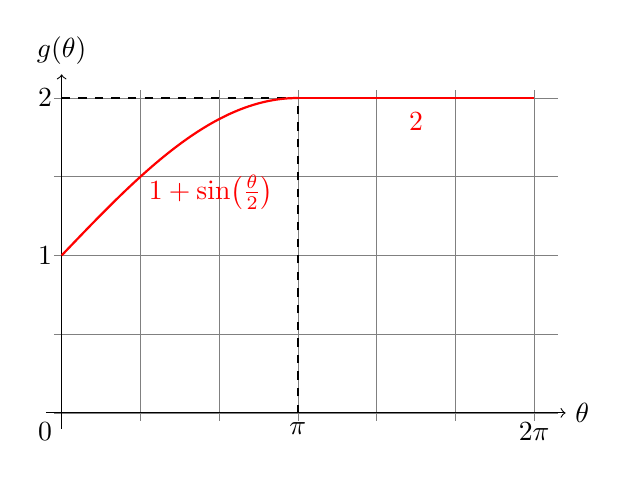
\begin{tikzpicture}
          \draw[very thin,color=gray] (-0.1,-0.1) grid (6.3,4.1);
          \draw[->] (-0.2,0) -- (6.4,0) node[right] {$\theta$}; 
          \draw[->] (0,-0.2) -- (0,4.3) node[above] {$g(\theta)$};
          \draw (0,0) node[below left] {$0$};
          \draw (0,2) node[left] {$1$};
          \draw (0,4) node[left] {$2$};
          \draw[dashed,thick] (0,4) -- (3,4);
          \draw (3,0) node[below] {$\pi$};
          \draw (6,0) node[below] {$2\pi$};
          \draw[dashed,thick] (3,0) -- (3,4);
          \draw[color=red,thick] plot[domain=0:3,smooth] (\x,{2+2*sin(\x r*3.14/6});
          \draw[color=red,thick] (1.9,2.8) node {$1+\sin(\frac{\theta}{2})$};
          \draw[color=red,thick] plot[domain=3:6,smooth] (\x,{4});
          \draw[color=red,thick] (4.5,3.7) node {$2$};
        \end{tikzpicture}
      \end{center}
      
      This is a consequence of results by \cite{Bae13}. We had done a direct proof of this, but it is not needed anymore since we have found a more general framework in section \ref{geoQubit} where we can deduce this value. It will be proved in the corollary \ref{corPureReal} page \pageref{corPureReal}.
      
      
      Since $g$ is concave, we have that $f_W$ is submodular:\\
      Let $S \subseteq T$ and $x \not\in T$, and let us order the $W_u$ in clockwise order and rename them with integers in $\set{1,\ldots,n}$:
      \begin{center}
        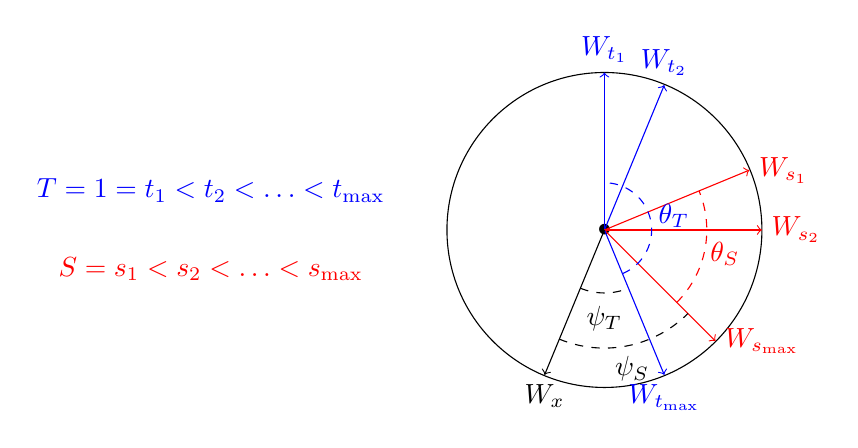
\begin{tikzpicture}
          \draw (0,0) coordinate (C) node {$\bullet$} circle (2);
          \draw[->, blue] (0,0) -- (0,2) coordinate (t1) node[above] {$W_{t_1}$};
          \draw[->,blue] (0,0) -- (0.76,1.84) node[above] {$W_{t_2}$};
          %\draw[blue] (1,1) node {$\ldots$};
          \draw[->, red] (0,0) -- (1.84,0.76) coordinate (s1) node[right] {$W_{s_1}$};
          \draw[->, red] (0,0) -- (2,0) node[right] {$W_{s_2}$};
          %\draw[red] (1.3,-0.5) node {$\ldots$};
          \draw[->, red] (0,0) -- (1.41,-1.41) coordinate (sM) node[below,right] {$W_{s_{\max}}$};
          %\draw[blue] (0.8,-1.2) node {$\ldots$};
          \draw[->,blue] (0,0) -- (0.76,-1.84) coordinate(tM) node[below] {$W_{t_{\max}}$};
          \draw[->] (0,0) -- (-0.76,-1.84) coordinate(k) node[below] {$W_x$};
          \draw[blue] (-5,0.5) node {$T = \set{1=t_1 < t_2 < \ldots < t_{\max}}$};
          \draw[red] (-5,-0.5) node {$S = \set{s_1 < s_2 < \ldots < s_{\max}}$};
          \draw[dashed,blue] pic["$\theta_T$", draw=blue, angle eccentricity=1.5, angle radius=0.6cm] {angle=tM--C--t1};
          \draw[dashed,red] pic["$\theta_S$", draw=red, angle eccentricity=1.2, angle radius=1.3cm] {angle=sM--C--s1};
          \draw[dashed] pic["$\psi_T$", draw=black, angle eccentricity=1.4, angle radius=0.8cm] {angle=k--C--tM};
          \draw[dashed] pic["$\psi_S$", draw=black, angle eccentricity=1.2, angle radius=1.5cm] {angle=k--C--sM};
          %\draw[dashed] pic["$\psi'_S$", draw=black, angle eccentricity=1.3, angle radius=1.2cm] {angle=s1--C--k};
        \end{tikzpicture}
      \end{center}


      If $t_1 \leq x \leq t_{\max}$, then the angle is unchanged: $\theta_{T \cup \set{x}}=\theta_T$, and so $f(T \cup \set{x}) = f(T)$, and in particular we have the submodular property for those instances.
      
      Otherwise, $x > t_{\max}$. We suppose that the angle $\psi_T$ between $W_x$ and $W_{t_{\max}}$ is smaller than the angle $\psi'_T$ between $W_x$ and $W_{t_1}$ (the analysis will be symmetric). Thus, we have that $\theta_{T \cup \set{x}} = \theta_T+\psi_T$.
      
      If the angle $\psi_S$ between $W_x$ and $W_{s_{\max}}$ is smaller than the angle $\psi'_S$ between $W_x$ and $W_{s_1}$, then $\theta_{S \cup \set{x}} = \theta_S+\psi_S$. By definition:
      \begin{equation}
        \begin{aligned}
          f(x|T) = g(\theta_{T \cup \set{x}})-g(\theta_T)\\
          f(x|S) = g(\theta_{S \cup \set{x}})-g(\theta_S)\\
        \end{aligned}
      \end{equation}

      \begin{lem}
        If $f$ is concave, we have that for all $a,b,c,d$ s.t. $c \geq a$ and $b-a \geq d-c \geq 0$:
        \[f(b)-f(a) \geq f(d)-f(c)\]
        \label{lemconcave}
      \end{lem}
      \begin{center}
        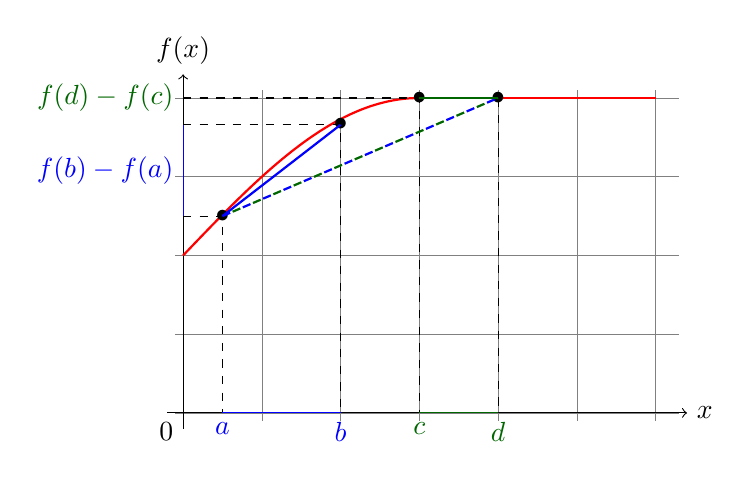
\begin{tikzpicture}
          \draw[very thin,color=gray] (-0.1,-0.1) grid (6.3,4.1);
          \draw[->] (-0.2,0) -- (6.4,0) node[right] {$x$}; 
          \draw[->] (0,-0.2) -- (0,4.3) node[above] {$f(x)$};
          \draw (0,0) node[below left] {$0$};
          \draw[color=red,thick] plot[domain=0:3,smooth] (\x,{2+2*sin(\x r*3.14/6});
          \draw[color=red,thick] plot[domain=3:6,smooth] (\x,{4});
          \draw[dashed] (0,2.5) -- (0.5,2.5) coordinate (A) node {$\bullet$} -- (0.5,0) node[blue,below] {$a$};
          \draw[dashed] (0,4) -- (3,4) coordinate (C) node {$\bullet$} -- (3,0) node[darkgreen,below] {$c$};
          \draw[dashed] (0,4) -- (4,4) coordinate (D) node {$\bullet$} -- (4,0) node[darkgreen,below] {$d$};
          \draw[dashed] (0,3.66) -- (2,3.66) coordinate (B) node {$\bullet$} -- (2,0) node[blue,below] {$b$};
          \draw[blue] (0.5,0) -- (2,0);
          \draw[darkgreen] (3,0) -- (4,0);
          \draw[thick,blue] (A) -- (B);
          %\draw[thick,blue] (B) -- (D);
          \draw[thick,blue,dash pattern= on 3pt off 5pt] (A) -- (D);
          %\draw[thick,darkgreen] (A) -- (C);
          \draw[thick,darkgreen] (C) -- (D);
          \draw[thick,darkgreen,dash pattern= on 3pt off 5pt,dash phase = 4pt] (A) -- (D);
          \draw[blue] (0,2.5) -- (0,3.66);
          \draw[blue] (0,3.08) node[left] {$f(b)-f(a)$};
          \draw[darkgreen] (0,4);
          \draw[darkgreen] (0,4) node[left] {$f(d)-f(c)$};
        \end{tikzpicture}
      \end{center}
      \begin{proof}
      Indeed, we have that $a \leq b \leq d$ and $a \leq c \leq d$. When we fix one point, since $f$ is concave, its slope is decreasing, so:
      \[\frac{f(b)-f(a)}{b-a} \geq \frac{f(d)-f(a)}{d-a} \text{ and } \frac{f(d)-f(a)}{d-a} \geq \frac{f(d)-f(c)}{d-c} \]

      So \[\frac{f(b)-f(a)}{b-a} \geq \frac{f(d)-f(c)}{d-c}\]
      But $b-a \geq d-c$ and thus we get that $f(b)-f(a) \geq \frac{b-a}{d-c}(f(d)-f(c)) \geq f(d)-f(c)$.
      \end{proof}
      We have that $\theta_{S \cup \set{x}} - \theta_S = \psi_S \geq \psi_T = \theta_{T \cup \set{x}} - \theta_T$ and $\theta_T \geq \theta_S$, so applying the lemma \ref{lemconcave}:
      \[g(\theta_{S \cup \set{x}})-g(\theta_S) \geq g(\theta_{T \cup \set{x}})-g(\theta_T)\]
      ie. $f(x|S) \geq f(x|T)$: we have the submodular property.

      
      Otherwise the angle $\psi'_S$ between $W_x$ and $W_{s_{1}}$ is strictly smaller than the angle $\psi_S$ between $W_x$ and $W_{s_{\max}}$. Then $\theta_{S \cup \set{x}} = \theta_S+\psi'_S$. But $\psi'_S \geq \psi'_T \geq \psi_T$ by hypothesis. So we can do the same analysis as before by replacing $\psi_S$ by $\psi'_S$. QED.
      
    \item Some of it was done in \cite{FSS19} (dimension 4 with real matrices).

      \begin{figure}[!h]
        \begin{center}
          \includegraphics[scale=0.25]{blochSphereCE.png}
          \caption{A counter-example of submodularity in the Bloch sphere for pure states}
          \label{BlochSphereCE}
        \end{center}
      \end{figure}
      
      Let us look now at the dimension 2 complex case. We define the following vectors (and their coordinates in the Bloch sphere), which are represented in figure \ref{BlochSphereCE} page \pageref{BlochSphereCE}:
      \begin{equation}
        \begin{aligned}
          \textcolor{blue}{\ket{\varphi} = \ket{0} = \pmqty{0\\0\\1}} && \textcolor{red}{\ket{\psi} = \ket{+} = \pmqty{1\\0\\0}}\\
          \textcolor{black}{\ket{\xi} =  \frac{1}{2}\pmqty{1\\-\sqrt{2}\\1}} && \textcolor{darkgreen}{\ket{\zeta} =  \frac{1}{2}\pmqty{-1\\\sqrt{2}\\-1}}\\
        \end{aligned}
      \end{equation}


      Then we take $W = \set{W_1,W_2,W_3,W_4} = \set{\dyad{\varphi},\dyad{\psi},\dyad{\xi},\dyad{\zeta}}$ and $S = \set{1,2}, T = S \cup \set{3}, x = 4$.\\
      We have that $f_W(S) = 1+\frac{\sqrt{2}}{2}$ using the value of $f_W$ for two vectors in the Bloch circle. Also, $f_W(T) < 2$ $(f_W(T) \simeq 1.976)$ since vectors are strictly in one hemisphere (we will see this result in section \ref{geoQubit}, also this was shown in \cite{Hunter04}).
      With the upcoming result, we will show that $f_W(S \cup \set{x}) = f_W(S) = 1+\frac{\sqrt{2}}{2}$. Finally, $f_W(T \cup \set{x}) = 2$ since it contains two orthogonal vectors $\ket{\xi}$ and $\ket{\zeta}$. Thus: \[f_W(x|S) = 0 < f_W(x|T) \simeq 0.024\]

      and so we have found our counterexample.
    \end{enumerate}

    \subsection{Other properties investigated}
    \begin{defi}[Approximate Submodularity, Weak Submodularity]
      Let $f : 2^X \rightarrow \mathbb{R}^+$ a nonnegative set function.
      \begin{enumerate}[label={(\arabic*)}]
      \item $f$ is said to be \emph{$\epsilon$-approximately submodular} \cite{KSC08,KC10} if
        \[ \forall S \subseteq T \subseteq X \text{ and } x \not\in T, f(x|S) \geq f(x|T) - \epsilon\]
      \item $f$ is said to be \emph{$\gamma$-weakly submodular} \cite{DK11,BBKT17} if
        \[ \forall \Omega,S, \underset{\omega \in \Omega - S}{\sum} f(\omega|S) \geq \gamma f(\Omega|S) \]
        We say that $\gamma_f$, the largest $\gamma$ such that $f$ is $\gamma$-weakly submodular, is the \emph{submodular ratio} of $f$.
      \end{enumerate}
    \end{defi}

    \begin{theo}[\cite{KSC08}]
      If $f$ is nonnegative, nondecreasing and  $\epsilon$-approximately submodular, then the greedy algorithm described in page \pageref{greedy} outputs $S_{\text{greedy}}$ of size $k$ approximating $S_{\text{opt}}$ such that:
      \begin{equation}
        \begin{aligned}
          f(S_{\text{greedy}}) \geq& \Big(1-\Big(1-\frac{1}{k}\Big)^k\Big)f(S_{\text{opt}}) - k\epsilon\\
          \geq& \Big(1-\frac{1}{e}\Big)f(S_{\text{opt}}) - k\epsilon
        \end{aligned}
      \end{equation}
    \end{theo}

    \begin{prop}[\cite{BBKT17}]
      If $f$ is nondecreasing, then:
      \begin{enumerate}[label={(\arabic*)}]
      \item $\gamma_f \in [0,1]$
      \item $f$ is submodular $\Leftrightarrow$ $\gamma_f = 1$
      \end{enumerate}
    \end{prop}
    
    \begin{theo}[\cite{BBKT17}]
      If $f$ is nonnegative, nondecreasing and $\gamma$-weakly submodular, then the greedy algorithm described in page \pageref{greedy} outputs $S_{\text{greedy}}$ of size $k$ approximating $S_{\text{opt}}$ such that:
      \begin{equation}
        \begin{aligned}
          f(S_{\text{greedy}}) \geq& \Big(1-\Big(1-\frac{\gamma}{k}\Big)^k\Big)f(S_{\text{opt}})\\
          \geq& \Big(1-\frac{1}{e^{\gamma}}\Big)f(S_{\text{opt}})
        \end{aligned}
      \end{equation}
    \end{theo}

    A notion of curvature is also described in \cite{BBKT17}, but useless for us as it seems that our function has always the worst case curvature.

    Mixing both properties, with small $\epsilon$ we get $\gamma_f$ not so far from $1$. It should be easy to prove that both bounds combine well. Also, using only one of those properties seems to fail.

    \newpage
    
    \section{Greedy algorithm}
We study now properly the problem of computing $S(W,k)$, adn finding the code $S$ that corresponds to this. As shown in \cite{BF17}, this problem is NP-complete already in the classical case and is even $(1-e^{-1})$-hard to approximate, and this approximation is obtained by the following simple greedy algorithm:
    
    \begin{algorithm}[H]
      \DontPrintSemicolon
      
      \KwInput{$k \in \set{1,\ldots,n}$}
      \KwOutput{An approximation of $S(W,k)$: A set $S \subseteq X$ of size at most $k$ that is \emph{close} to maximize $f_W(S)$ over all of those sets}
      \KwData{$W = \set{W_1,\ldots,W_n}$}
      $S = \emptyset$\\
      \For{$i \in \set{1,\ldots,k}$}
         {
           $x^* = \underset{x \in X-S}{\text{argmax }} f_W(x|S)$\\
           $S = S \cup \set{x^*}$
         }

         \Return $S$
         \caption{Greedy algorithm}
         \label{greedy}
    \end{algorithm}

    \subsection{Classical case}
    In fact, this algorithm in the classical case gives a $(1-(1-\frac{1}{k})^k)$-approximation for the problem of size $k$ since in that case $f_W$ is submodular \cite{BF17}. We have found in particular a series of explicite examples where this bound is obtained, which shows the tightness of this approximation:
    
    For $k=2$, this is obtained by the matrix $W^2$ (where line $i$ corresponds to the diagonal coefficients of $W^2_i$, since we are in the classical case):
    \[W^2 = \pmqty{\frac{1}{2} & \frac{1}{2}\\1 & \\ & 1}\]
    The greedy algorithm gives the set $S_{\text{greedy}}=\set{1,2}$ whose value is $f_{W^2}(S_{\text{greedy}})=3/2$ as answer, whereas the optimal value is $f_{W^2}(S_{\text{opt}}=\set{2,3}) = 2$. This gives an approximation ratio of:
    \[\frac{f_{W^2}(S_{\text{greedy}})}{f_{W^2}(S_{\text{opt}})}= \frac{3}{4} = 1-\Big(1-\frac{1}{2}\Big)^2\]
    
    For $k=3$:
    \[W^3= \pmqty{\frac{1}{3} &  & \frac{1}{3} &  & \frac{1}{3} & \\\frac{1}{3} & \frac{2}{9} &  & \frac{2}{9} &  & \frac{2}{9}\\\frac{1}{2} & \frac{1}{2} &  &  &  & \\ &  & \frac{1}{2} & \frac{1}{2} &  & \\ &  &  &  & \frac{1}{2} & \frac{1}{2}\\}\]
    We get:
     \[\frac{f_{W^3}(S_{\text{greedy}}=\set{1,2,3})}{f_{W^3}(S_{\text{opt}}=\set{3,4,5})}= \frac{19/9}{3} = \frac{19}{27} = 1-\Big(1-\frac{1}{3}\Big)^3\]
     These first two cases were found by Daniel Szylagyi. We have generalized those examples for all $k$. We need the dimension $d=\frac{k(k-1)}{2}$ (number of columns) and the number of states $n=2k-1$ (number of lines). Then we define the matrix $W^k = \pmqty{G\\O}$ in the following way with:
     \[G = \pmqty{U & V & \ldots & V}\]
     where V is repeated $(k-1)$ times and $U,V$ of size $(k-1) \times k $ defined by:
     \[U = \pmqty{u^k_1 & 0 & \ldots & 0 \\
       u^k_1 & u^k_2 & \ddots & 0 \\
       \vdots & \vdots & \ddots & \vdots \\
       u^k_1 & u^k_2 & \ldots  & u^k_{k-1} \\
     }\]
     \[V = \pmqty{\dmat[0]{u^k_1,\ddots, u^k_{k-1}}}\]


     and where the sequence $(u^k_j)_{j \in \mathbb{N^*}}$ is defined in the following way:

     \[(u^k_j)_{j \in \mathbb{N^*}} : \begin{cases}
      u^k_1 = \frac{1}{k}\\
      u^k_{j+1} = u^k_j + \frac{1-u^k_j}{k}\\
      \end{cases}
      \]

      and we define $O$:
      
     \[O = \pmqty{\frac{1}{k-1} & \ldots &\frac{1}{k-1} & 0 && \ldots & \ldots && 0\\
       0 & \ldots & 0 & \frac{1}{k-1} & \ldots &\frac{1}{k-1} &  0 & \ldots & 0\\
       \vdots  && \vdots && \ddots && \vdots && \vdots\\
       0 && \ldots & \ldots && 0 &\frac{1}{k-1} & \ldots &\frac{1}{k-1}\\
     }\]
     where O has $k$ lines and each $\frac{1}{k-1}$ is repeated $k-1$ times.

     We can show by induction on $j$ that:
     \[u^k_j = \frac{\overset{j-1}{\underset{i=0}{\sum}}(-1)^{j-1-i}\pmqty{j\\i}k^i}{k^j}\]

     and:

     \[\frac{f_{W^k}(\set{1,\ldots,j})}{k} =  u^k_j\]
     
     We deduce from this that:
     \begin{equation}
       \begin{aligned}
         \frac{f_{W^k}(S_{\text{greedy}}=\set{1,\ldots,k})}{f_{W^k}(S_{\text{opt}}=\set{k,\ldots,2k-1})} &=&& \frac{f_{W^k}(\set{1,\ldots,k})}{k} =  u^k_k\\ &=&& \frac{\overset{k-1}{\underset{i=0}{\sum}}(-1)^{k-1-i}\pmqty{k\\i}k^i}{k^k}\\
         &=&& \frac{k^k-(k-1)^k}{k^k} = 1-\Big(1-\frac{1}{k}\Big)^k
       \end{aligned}
     \end{equation}
     
     For now, we do not write here precise proofs which are technical but not difficult.

     \subsection{Pure real quantum case}
     \subsubsection{NP-hardness and inapproximability}
     We show in this section that the problem we are trying to solve with the greedy algorithm is NP-hard, even restricted to pure real states. However, the NP-hardness comes for different reasons than in the classical case.

     \begin{theo}
       The following decision problem is NP-hard:

       \begin{description}
         \item[\underline{Problem:}] \emph{PureRealChannelCoding}
         \item[\underline{Instance:}] A finite set of $W$ of pure real states $W_i$ (real, rank one states) of size $n$, $M \in \mathbb{R}$ and $k \in \set{1,\ldots,n}$
         \item[\underline{Question:}] Does $S(W,k) \geq M$ ?
       \end{description}
     \end{theo}

     \begin{proof}
       Inspired by a proof in \cite{CMi09}, we give a reduction from \emph{Exact cover by 3-sets} which is known to be NP-complete (see for instance \cite{GJ79}):

       \begin{description}
         \label{X3C}
         \item[\underline{Problem:}] \emph{Exact cover by 3-sets (X3C)}
         \item[\underline{Instance:}] A set $Q$ and a collection $C$ of 3-elements subsets of $Q$
         \item[\underline{Question:}] Does there exists an exact cover for $Q$, i.e. a sub-collection $S$ of indices of $C$ such that every element in $Q$ appears \emph{exactly} once in $\set{c_x}_{x \in S}$ ?
       \end{description}

       We use the following reduction. Let $Q = \set{q_1,\ldots,q_m}$ and $C = \set{c_1,\ldots,c_n}$.
       We take $k=\ceil{\frac{m}{3}}$, $M=1$, and $W = \set{A^{(j)}(A^{(j)})^T,j \in \set{1,\ldots,n}}$, where $A^{(j)}$ is the $j$-th column of $A$ which is a $m \times n$ real matrix defined by:

       \[A_{i,j} = \begin{cases}
         \frac{1}{\sqrt{3}} \text{ if } q_i \in c_j\\
         0 \text{ otherwise}\\
       \end{cases}
       \]

       First, each $A^{(j)}$ is indeed a unit vector of $\mathbb{R}^m$ since for each $j$, $c_j$ contains exactly $3$ elements of $Q$ since we have taken a valid instance of \emph{X3C}. Thus we have defined a valid instance of \emph{PureRealChannelCoding}.

       Let us show that there exists an exact cover for $Q$ if and only if $S(W,k) \geq M$.

       \begin{itemize}
       \item[$(\Rightarrow)$] If there is an exact cover $S$ for $Q$, then $\abs{S}=\frac{m}{3} \in \mathbb{N}$. We have then that $\abs{S}=k$ and we will show that $f_W(S) \geq k$, which implies that $S(W,k) \geq \frac{f_W(S)}{k} = 1 = M$. Indeed, since $S$ is an exact cover, there is exactly one non-zero coefficient in each line of $\set{A^{(j)},j \in S}$ seen as a matrix. Thus, we take as POVM $(\Lambda_j)_{j \in S}$ defined by:
         \[\Lambda_j = \underset{i:A^{(j)} \not= 0}{\sum} \dyad{i} = \underset{i:q_i \in c_j}{\sum} \dyad{i} \]
         which is in fact a PVM. Indeed, $\Lambda_j \succcurlyeq 0$ and:
         \[\underset{j \in S}{\sum} \Lambda_j = \underset{j \in S}{\sum} \underset{i:q_i \in c_j}{\sum} \dyad{i} =  \underset{j \in Q}{\sum} \dyad{i} = \mathbbm{1}\]

         since $S$ is an exact cover for $Q$.

         Thus:
         \begin{equation}
           \begin{aligned}
             f_W(S) \geq& \underset{j \in S}{\sum} \Tr(\Lambda_j W_j) = \underset{j \in S}{\sum} \Tr(\underset{i:A^{(j)} \not= 0}{\sum} \dyad{i} A^{(j)}(A^{(j)})^T)\\
             =&  \underset{j \in S}{\sum} \underset{i:A^{(j)}_i \not= 0}{\sum} \Tr(\dyad{i} A^{(j)}(A^{(j)})^T) = \underset{j \in S}{\sum} \Tr(A^{(j)}(A^{(j)})^T)\\
             =& \underset{j \in S}{\sum} 1 = \abs{S} = k
           \end{aligned}
         \end{equation}
     
       \item[$(\Leftarrow)$] Suppose that $S(W,k) \geq M$. We have in fact that $S(W,k) = M$. Indeed for all $S$ of size at most $k$, we have that $f_W(S) \leq k$ as seen in property \ref{smallprops}, and so $S(W,k) \leq 1 = M$.

         Let $S$ be a set such that $f_W(S) = k$ (and so $\abs{S}=k$). To obtain such a value, necessarly for all $j$ in $S$, $\Lambda_j$ needs to be at least a projector on $W_j$, otherwise we have that $\Tr(\Lambda_j W_j) < \Tr(W_j) = 1$. Thus:
         \[\Lambda_j \succcurlyeq \Pi_{\text{vect}\set{A^{(j)}}} = \Pi_{\text{vect}\set{\ket{i}, i:q_i \in c_j}} = \underset{i:q_i \in c_j}{\sum} \dyad{i}\]

         And so:
         \[\mathbbm{1} = \underset{j \in S}{\sum} \Lambda_j \succcurlyeq \underset{j \in S}{\sum}\underset{i:q_i \in c_j}{\sum} \dyad{i}\]

         but $S$ is of size $k = \ceil{\frac{m}{3}}$, and each $c_j$ is of size 3, so there are $3*\ceil{\frac{m}{3}}$ in that previous sum. If $\frac{m}{3} \not\in \mathbb{N}$, then $3*\ceil{\frac{m}{3}} > m$, which is a contradiction with the previous inequality since $(\ket{i})_{i \in [m]}$ is a basis of $\mathbb{R}^m$. Thus $\frac{m}{3} \in \mathbb{N}$, there are exactly $m$ terms in the previous sum and we have the equality $\Lambda_j = \underset{i:q_i \in c_j}{\sum} \dyad{i}$, which means that $S$ is an exact cover of $Q$ since there can't be any overlap.
       \end{itemize}
     \end{proof}

     A consequence of the precedent proof is the hardness of approximation of our problem. If there is an overlap of one coordinate of two vectors in the previous reduction, we get numerically that the value of $f_W(S)$ is decreased by $C_{\text{hard}} \simeq 0.05719$. Thus we have:

     \begin{cor}
       The optimization version of \emph{PureRealChannelCoding}, which consists in computing $S(W,k)$, is NP-hard to approximate within a factor $1-\frac{C_{\text{hard}}}{k} + \epsilon$ for $\epsilon > 0$. So there does not exist a FPTAS that solves this problem if $P \not= NP$ (it fails if relative error is asked to be smaller than $\frac{C_{\text{hard}}}{n}$ since $k \leq n$).
     \end{cor}
     
     \subsubsection{Best counter-example to the greedy algorithm}
     The greedy algorithm still seems to work: we have not been abled yet to find a counter-example to this ratio of approximation, although the precedent proof doesn't work since our function is not submodular in this broader case.

     We will depict here the best counter-example we have been able to find so far.

     We place ourselves in $\mathbb{R}^k$, where states are unit vectors.
     First we take a squeezed orthonormal basis:
     \[ \ket{i'} = \sqrt{1-\epsilon}\ket{i} + \sqrt{\frac{\epsilon}{k-1}}\underset{j \not= i}{\sum}\ket{j}\]
     where $\ket{1},\ldots,\ket{k}$ is the orthonormal basis and $\epsilon > 0$.

     We construct a sequence $S_1,\ldots,S_k$ and $\ket{g_1},\ldots,\ket{g_k}$ in the following way:
     \[S_j = \set{\ket{j'},\ket{(j+1)'},\ldots,\ket{k'}}\]
     And in particular:
     \[S_1 = \set{\ket{1'},\ldots,\ket{k'}}\]
     
     Let O be the origin of $\mathbb{R}^k$. Take $\ket{g_1}$ the unique point at the same distance of all of points of $S_1$. Thus:
     \[\ket{g_1} = \frac{1}{\sqrt{k}}\underset{i}{\sum}\ket{i'} = \frac{1}{\sqrt{k}}\underset{i}{\sum}\ket{i}\]

     \begin{algorithm}[H]
      \DontPrintSemicolon
      $C = O$\\
      $H = \mathbb{R}^k$\\
      $\ket{g_1} = \frac{1}{\sqrt{k}}\underset{i}{\sum}\ket{i'} = \frac{1}{\sqrt{k}}\underset{i}{\sum}\ket{i}$\\
      \For{$j \in \set{1,\ldots,k-1}$}
         {
           $L = C + \text{vect}\set{\overrightarrow{n}}$ affine line where $\overrightarrow{n} = \frac{\overrightarrow{\ket{g_j}} - \overrightarrow{OC}}{\norm{\overrightarrow{\ket{g_j}} - \overrightarrow{OC}}}$\\
           $H =$ only affine hyperplane containing all points of $S_j$ : $\overrightarrow{n}$ is a normal vector of $H$ \\
           $P = H \cap L$ which is a point, we get it by the formula:
           \[P = C + ((\overrightarrow{\ket{j'}} - \overrightarrow{OC}) \cdot \overrightarrow{n})\overrightarrow{n}\]
           \\
           $C = P$ our new center\\
           $\ket{g_{j+1}} = $ central symmetry of $\ket{j'}$ around $C$ which is given by:
           \[\overrightarrow{\ket{g_{j+1}}} = 2 \times \overrightarrow{OC}-\overrightarrow{\ket{j'}}\]
         }

         \Return $\set{\ket{g_1},\ldots,\ket{g_{k-1}}}$
         \caption{Counter-example to our greedy algorithm}
    \end{algorithm}

      \begin{figure}[!h]
        \begin{center}
          \includegraphics[scale=0.25]{CEgreedypure.png}
          \caption{The construction of $g_1$ and $g_2$ (in red) for the case $k=3$ (\emph{one}, \emph{two} and \emph{three} correspond respectively to $\ket{1'},\ket{2'}$ and $\ket{3'}$) where we have taken $\epsilon=0.1$}
          \label{CEgreedypuredim3}
        \end{center}
      \end{figure}
      \begin{figure}[!h]
        \begin{center}
          \includegraphics[scale=0.25]{CEgreedyProjDim4.png}
          \caption{We have represented for $k=4$ what happened after the first projection on $H$ of dimension 3 in order to find $g_2$ (in red), where the $4$ black points are the elements of $S_1$. Note that the center $C$ here is different from $O$ which does not belong to $H$ (see figure \ref{CEgreedypuredim3} page \pageref{CEgreedypuredim3} for instance)}
          \label{CEgreedypuredim4}
        \end{center}
      \end{figure}

      In figure \ref{CEgreedypuredim3} page \pageref{CEgreedypuredim3}, we see how we construct $g_1$ and $g_2$. We see also that it is recursive: the way we construct $g_2$ for $k=3$ is the same as the construction of $g_1$ for $k=2$ when we stay inside the hyperplane $H$. In particular, we see also this in figure \ref{CEgreedypuredim4} page \pageref{CEgreedypuredim4} where we show only the first projection and we see that getting $g_2$ here is the same as getting $g_1$ in dimension $3$ and so on.
      
      We take then $W = \set{\dyad{g_1}, \ldots, \dyad{g_{k-1}}, \dyad{1'}, \ldots, \dyad{k'}}$. The greedy algorithm takes $S_{\text{greedy}} = \set{\dyad{g_1}, \ldots, \dyad{g_{k-1}}, \dyad{(k-1)'}}$ whereas the optimal solution is to take $S_{\text{opt}} = \set{\dyad{1'}, \ldots, \dyad{k'}}$.

      Numerically, the best parameters in order to minimize the efficiency of our greedy algorithm are the following for small dimensions ($k \leq 10$): $k=4$ and $\epsilon=0.199$. Then:

      \[\frac{f_W(S_{\text{greedy}})}{f_W(S_{\text{opt}})} \simeq 0.753 > 1-\Big(1-\frac{1}{4}\Big)^4 \simeq 0.684\]
\end{proof}

\newpage

\section{Interpretation of our problem in terms of convex shape covering}
\subsection{Generalized Probabilistic Theories (GPTs)}
Introduced in \cite{Barrett07}, GPTs are a generalization of classical and quantum theories into a more general framework where we consider any convex body as the set of states, and we look at the cone spanned by this space. One of the motives of these theories is to better understand the critical properties of quantum theory, such as entanglement.

\begin{figure}[!h]
  \begin{center}
    \includegraphics[scale=0.25]{GPT.png}
    \caption{The basic ingredients of a GPT are a real finite-dimensional vector space $V$ and a cone $C$. The order unit functional $u$ defines a hyperplane $u^{-1}(1)$, whose intersection with $C$ identifies the state space $\Omega$.}
    \label{GPT}
  \end{center}
\end{figure}

\begin{itemize}
\item Formally, a \emph{GPT} is a triple $(V, C, u)$, where $V$ is a finite-dimensional real vector space, $C \subset V$ is a proper cone, and the \emph{order unit} $u \in $ int$(C^*)$ is a strictly positive convex-linear functional on $C$: $\forall x \in C-\set{0}$, $u(x) > 0$.

\item A subset $C \subseteq V$ is called a \emph{cone} if $\lambda C = C$ for all $\lambda > 0$. A cone is said to be pointed if $C \cap (-C) = \set{0}$, generating if $C - C = $ span$(C) = V$, and \emph{proper} if it is convex, topologically closed, pointed, and generating. Mathematically, this gives $V$ the structure of an \emph{ordered vector space}: the ordering is defined for $x, y \in V$ by saying that $x \leq_C y$ if $y - x \in C$.

\item Positive functionals on $C$ in the dual space $V^*$ form the dual cone $C^*$. If $C$ is proper, then $C^{**} = C$ modulo the identification $V^{**} = V$. We can extend there the order in $C$ for elements of $V^*$: $f \leq_{C^*} g$ if $f(x) \leq_C g(x)$ for all $x \in C$.

\item A \emph{classical} cone $C$ is one that is generated by a basis of $V$ , ie. $C = \set{\sum_i \lambda_i e_i : \forall i, \lambda_i \geq 0}$ for some basis $\set{e_i}_i$.

\item A natural way to construct a cone is through one of its sections. Namely, given a convex set $K \subseteq V$, let us define the cone $\mathcal{C}(K) = \set{(tx, t) : x \in K, t \in \mathbb{R}^+ } \subseteq V \times \mathbb{R}$. One can verify that $\mathcal{C}(K)$ is a proper cone if and only if $K \subset V$ is a \emph{convex body} (compact convex set with non-empty interior), and that it is non-classical if and only if $K$ is not a simplex. Moreover, every proper cone in dimension $d$ is linearly isomorphic to $\mathcal{C}(K)$ for some $(d-1)$-dimensional convex body $K$

\item The \emph{state space} is defined as $\Omega := C \cap u^{-1}(1)$. It is the base of $C$, ie. $C = \set{\lambda \omega : \lambda \geq 0, \omega \in \Omega}$, such that $\forall \omega \in \Omega, u(\omega) = 1$.

\item A \emph{measurement} is a finite collection of \emph{effects} $(e_i)_{i \in I}$ such that $e_i \in V^*$ satisfies $e_i \geq_{C^*} 0$ and $\sum_{i \in I} e_i = u$ (so in particular $0 \leq_{C^*} e \leq_{C^*} u$). The probability of obtaining the outcome $i$ when measuring the state $\omega$ is $e_i(\omega) \in [0,1]$.
\end{itemize}

For example, regular quantum theory can be restated in terms of a GPT in the following way:
\begin{itemize}
\item $V := \mathcal{H}_d$ is the real vector space.
\item $C := $ PSD$_d = \set{M \in \mathcal{H}_d : M \succcurlyeq 0}$ is the cone.
\item $u := \Tr = \Tr(\mathbbm{1} \cdot) = \langle \mathbbm{1}, \cdot \rangle$ is the order unit, and it can be identified to $\mathbbm{1}$ through the scalar product $\langle A, B \rangle := \Tr(A^{\dagger}B)$ and the associated isomorphism between $V^*$ and $V$. Inequalites $\leq_{C^*}$ become $\leq_C$ through this isomorphism.
\item In particular, $\Omega = C \cap u^{-1}(1) = \set{M \in \mathcal{H}_d : M \succcurlyeq 0 \text{ and } \Tr(M) = 1} = \mathcal{D}_d$ the usual space state. An effect $e \in V^*$ is such that $0 \leq_{C^*} e \leq_{C^*} u$. Through the previous isomorphism, it can be identified to $0 \preccurlyeq \Lambda_e \preccurlyeq \mathbbm{1}$, and the probability of the measuring $e$ becomes $e(M) = \langle \Lambda_e, M \rangle = \Tr(\Lambda_e^{\dagger}M)$. A measurement is a finite set of such effects $(e_i)_{i \in I}$ such that $\sum_{i \in I} e_i = u$. Through this isomorphism, this translate to the usual definition of a POVM: a finite set of positive operators $(\Lambda_{e_i})_{i \in I}$ such that $\sum_{i \in I} \Lambda_{e_i} = \mathbbm{1}$.
\end{itemize}

\subsection{Generalization of the channel coding problem in a GPT}
We study here our channel coding problem in a GPT $(V,C,u)$ (and $\Omega$ state space). We suppose we have $\set{W_x}_{x \in X} \subseteq \Omega$, and we define:
\begin{defi}[General Channel Coding Function]
  \begin{equation}
    \begin{aligned}
      &f_W(S) :=&& \underset{(e_x)_{x \in S}}{\maxi} &&\underset{x \in S}{\sum} e_x(W_x) \\
      &&& \st && \underset{x \in S}{\sum} e_x = u \\
      &&&&& e_x \geq_{C^*} 0, \forall x \in S
    \end{aligned}
  \end{equation}
\end{defi}

\begin{prop}
  We can replace $\underset{x \in S}{\sum} e_x = u$ by $\underset{x \in S}{\sum} e_x \leq_{C^*} u$.
\end{prop}

This is a conic program, we can compute its dual through the Lagrangian as it is done in \cite{BKK16}. We have also strong duality in this general case so:

\begin{prop}[Strong Duality]
  \begin{equation}
    \begin{aligned}
      &f_W(S) =&& \underset{\rho}{\mini} && u(\rho) \\
      &&& \st && \rho \geq_C  W_x, \forall x \in S
      \end{aligned}
  \end{equation}
\end{prop}

\begin{rk}
  If the input data is not uniform, but rather follows the probabilities $(q_x)_{x \in S}$, then the primal objective becomes $\sum_{x \in S} q_x\abs{S}e_x(W_x)$, and dual constraints become $\rho \geq_C q_x\abs{S} W_x$.
\end{rk}

\begin{defi}[Channel Coding Optimization]
  \[ S(W,k) := \frac{1}{k} \underset{S \subseteq X, \abs{S} \leq k}{\max} f_W(S) \]
\end{defi}

\begin{rk}
  \begin{enumerate}
  \item $\rho$ won't be always unique: it will depend on the shape of the convex body $\Omega$.
  \item If we can compute efficiently one instance of this problem, we can use the same greedy algorithm as defined in algorithm \ref{greedy} to approximate in polynomial time $S(W,k)$. One of the fundamental questions we want to solve is to understand for which shapes this algorithm gives a good approximation.
  \item We can also define a relaxation of the dual problem as in \cite{FSS19}, and the method to transform one of its solutions to the original dual problem. However we can't analyse its efficiency with the same arguments as in the quantum case. Another question we want to solve is whether this is efficient and for which shapes.
  \end{enumerate}
\end{rk}


\subsection{Equivalence with the minimum enclosing convex shape problem (MECP)}
\begin{defi}[MinEffect]
  For a GPT $(V,C,u)$, it is the following conic problem:
  \begin{equation}
    \begin{aligned}
      &f_W(S) =&& \underset{\rho}{\mini} && u(\rho) \\
      &&& \st && \rho \geq_C  W_x, \forall x \in S
      \end{aligned}
  \end{equation}
\end{defi}

\begin{defi}[Minimum Enclosing Convex Problem (MECP) \cite{BK13}]
  $\Gamma \subseteq \mathbb{R}^n$ convex body that contains $0$, $P \subseteq -\Gamma$ finite set of points, find the least dilatation factor $r \geq 0$, such that a translate of $r\Gamma$ contains $P$:
  \begin{equation}
    \begin{aligned}
      R(P,\Gamma) := && \mini &&& r\\
      && \st &&& P \subseteq \mathcal{D}_{\Gamma}(\gamma,r) := \gamma + r\Gamma \\
      && &&& \gamma \in \mathbb{R}^n, r \geq 0
    \end{aligned}
  \end{equation}
\end{defi}

\begin{rk}
  Since the problem is translation invariant, and a dilatation of $\Gamma$ can be found directly on the coefficient $r$, we could have stated MECP with $\Gamma \not\ni 0$ and $P \subseteq \mathbb{R}^n$.
\end{rk}

\begin{defi}[Lower Cone]
  For a GPT $(V,C,u)$, the lower cone $\mathcal{C}_{\leq_C}(x)$ of an element $x \in V$ is defined by:
  \[ \mathcal{C}_{\leq_C}(x) := \set{y \in V \text{ s.t. } y \leq_C x}\]
\end{defi}

\begin{rk}
  $\mathcal{C}_{\leq_C}(x)$ is an (affine) proper cone of vertex $x$
\end{rk}

For some fixed $c \in \Omega$, we define $\Omega_c := \Omega - c$ the translation of $\Omega$ in the direction $c$. In particular, $\Omega_c \subseteq u^{-1}(0)$ by linearity of $u$.

\begin{prop}
  For $x \in V$ such that $r_x := u(x) > 0,  \mathcal{D}(x):=\mathcal{D}_{-\Omega_c}(x - r_xc ,r_x) = x - r_x\Omega$ is a base of $\mathcal{C}_{\leq_C}(x)$  included in $u^{-1}(0)$. 
  \label{propbase}
\end{prop}

\begin{proof}
  $\mathcal{D}(x) \subseteq u^{-1}(0)$ by linearity of $u$. Let us show that $\mathcal{D}(x)$ is a base of $\mathcal{C}_{\leq_C}(x)$, ie. $\mathcal{C}_{\leq_C}(x)=x+\mathbb{R}^+(\mathcal{D}(x)-x)$. Let $y \in \mathcal{C}_{\leq_C}(x)$, ie. $y \leq_C x$. Suppose that $y \not= x$ ($x = x + 0$ otherwise), ie. $y <_C x$. Then $\frac{1}{u(x-y)}(x-y)$ is a state so:
  \[y_0 = x - \frac{r_x}{u(x-y)}(x-y) \in \mathcal{D}(x)\]

  Then $y = x + \frac{u(x-y)}{r_x}(y_0-x)$ so $\mathcal{C}_{\leq_C}(x) \subseteq x+\mathbb{R}^+(\mathcal{D}(x)-x)$.

  On the other hand, let us take $y \in x+\mathbb{R}^+(\mathcal{D}(x)-x)$: there exist $k \in \mathbb{R}^+$ and $z \in \Omega$ such that $y = x + k[(x-r_xz)-x] = x - kr_xz$. But $kr_xz \geq_C 0$ since $k,r_x \geq 0$ and $z \in \Omega \subseteq C$, so $y = x - kr_xz \leq_C x$, ie. $x+\mathbb{R}^+(\mathcal{D}(x)-x) \subseteq \mathcal{C}_{\leq_C}(x)$.
\end{proof}

We show in the following sections that both problems MinEffect and MECP are equivalent.

\begin{subsubsection}{MinEffect $\rightarrow$ MECP}
  We consider a MinEffect instance, ie. a GPT $(V,C,u)$, $\Omega = C \cap u^{-1}(1)$ the state space and a finite set of states $\set{W_x}_{x \in S} \subseteq \Omega$. Let $c \in \Omega$ a reference state we call the center state. We define the following MECP instance:
  \begin{itemize}
  \item $\Gamma := -\Omega_c \subseteq u^{-1}(0) = \mathbb{R}^n$ modulo a choice of a basis, since $V$ is a real finite dimension vector space. $0 = -(c-c) \in \Gamma$ since $c \in \Omega$.
  \item $P := \set{W_x-c}_{x \in S} \subseteq \Omega_c = -\Gamma $ with the same basis choice.
  \end{itemize}

  We define:
  \begin{prop}
  \begin{equation}
    \begin{aligned}
      \varphi : && \mathbb{R}^n\times \mathbb{R}^+ &&\rightarrow&&& V\\
      && (\gamma,r) &&\mapsto&&& \gamma + (r+1)c
    \end{aligned}
  \end{equation}
  is a bijection with $\varphi^{-1}(x)=(x-(u(x)-1)c,u(x)-1)$
  \end{prop}

  \begin{theo}
    $(\gamma,r)$ is an optimal solution of MECP if and only if $\varphi(\gamma,r)$ is an optimal solution of MinEffect for the instances we have described.
    \label{eqtheo}
  \end{theo}

  \begin{proof}
    Let $(\gamma,r) \in \mathbb{R}^n\times \mathbb{R}^+$. If $r>0$, $\mathcal{D}_{-\Omega_c}(\gamma,r)$ is a basis of $\mathcal{C}_{\leq_C}(\varphi(\gamma,r)-c)$ included in $u^{-1}(0)$ by property \ref{propbase}. In particular, we have that for $y \in u^{-1}(0)$, $y \in \mathcal{D}_{-\Omega_c}(\gamma,r)$ if and only if $y \leq_C \varphi(\gamma,r) - c$, which is trivially true when $r=0$. Thus in particular, $W_x - c \in \mathcal{D}_{-\Omega_c}(\gamma,r) \iff W_x \leq_C \varphi(\gamma,r)$

    Thus, $P \subseteq \mathcal{D}_{-\Omega_c}(\gamma,r) \iff W_x \leq_C \varphi(\gamma,r), \forall x \in S$, and $u(\varphi(\gamma,r)) = r+1$ and $r_{\varphi^{-1}(x)} = u(x)-1$, so we minimize the same parameter up to a constant $1$. Furthermore $\varphi$ is a bijection between the variable spaces: with the previous equivalence it means that it maps MECP feasible solution to MinEffect feasible solution and reciprocally. Since we minimize the same parameter through $\varphi$, it maps optimal solutions of MECP to optimal solutions of MinEffect and reciprocally.
  \end{proof}
\end{subsubsection}

\begin{subsubsection}{MECP $\rightarrow$ MinEffect}
  We consider a MECP instance $(\Gamma,\set{P_x}_{x \in S}) \subseteq \mathbb{R}^n \times -\Gamma$ and $0 \in \Gamma$. We define a MinEffect instance composed of a GPT $(V,C,u)$ and a set of states $W \subseteq \Omega = C \cap u^{-1}(1)$ in the following way:
  \begin{itemize}
  \item $V := \mathbb{R}^{n+1}$
  \item $C := \set{(tx,t) : x \in -\Gamma, t \in \mathbb{R}^+}$
  \item $\begin{aligned}
      u : && \mathbb{R}^n \times \mathbb{R} &&\rightarrow&&& \mathbb{R}\\
      && (x,t) &&\mapsto&&& t
    \end{aligned}$

  \item So, in particular, $\Omega = C \cap  u^{-1}(1) = \set{(x,1) : x \in -\Gamma}$
  \item $W := \set{(P_x,1)}_{x \in S} \subseteq \Omega$
  \item We define $c:=(0,\ldots,0,1) \in \Omega$ (since $0 \in \Gamma$) and we get then that $\Gamma = -\Omega_c$ if we see $\Gamma$ living in $\mathbb{R}^{n+1}$. Thus $P \subseteq \Omega_c = -\Gamma$.
  \end{itemize}

  \begin{theo}
    $(\gamma,r)$ is an optimal solution of MECP if and only if $(\gamma,r+1)$ is an optimal solution of MinEffect for the instances we have described.
  \end{theo}
  
  \begin{proof}
    It is exactly the same proof as in theorem \ref{eqtheo}.
  \end{proof}
\end{subsubsection}

\begin{subsubsection}{Non-uniform inputs case}
  In this section we do not suppose anymore that we have uniform input. Thus the dual problem to compute our Channel Coding function becomes:
  \begin{defi}[MinEffect$^*$]
    For a GPT $(V,C,u)$, it is the following conic problem:
    \begin{equation}
    \begin{aligned}
      &f_W(S) =&& \underset{\rho}{\mini} && u(\rho) \\
      &&& \st && \rho \geq_C  W_x, \forall x \in S
      \end{aligned}
    \end{equation}
    where we require only $W_x \geq_C 0$: $u(W_x)$ is only known to be nonnegative.
  \end{defi}

  We also define a variant of MECP:
  \begin{defi}[Generalized Minimum Enclosing Convex Problem (MECP$^*$)]
  $\Gamma \subseteq \mathbb{R}^n$ convex body that contains $0$, $P \subseteq \underset{\lambda \geq 0}{\bigsqcup}\set{\alpha + \lambda\Gamma,  \alpha \in \mathbb{R}^n}$ finite set of dilatations of $\Gamma$,  find the least dilatation factor $r \geq 0$, such that a translate of $r\Gamma$ contains $P$:
    \begin{equation}
    \begin{aligned}
      R(P,\Gamma) := && \mini &&& r\\
      && \st &&& p \subseteq \mathcal{D}_{\Gamma}(\gamma,r) := \gamma + r\Gamma, \forall p \in P\\
      && &&& \gamma \in \mathbb{R}^n, r \geq 0
    \end{aligned}
  \end{equation}
  \end{defi}

  Instead of having only points, we have also dilations of $\Gamma$ to cover with $\Gamma$.
  
  Let us consider the points $W_x$. Each of them generates a cone $\mathcal{C}_{\leq_C}(W_x)$ with a base in $u^{-1}(0)$ given by $\mathcal{D}(W_x)=\mathcal{D}_{-\Omega_c}(W_x - u(W_x)c ,u(W_x)) = W_x - u(W_x)\Omega$ by property \ref{propbase}. We transform an instance of MinEffect$^*$ to MECP$^*$ by taking $P = \set{\mathcal{D}(W_x)}_{x \in S}$ and reciprocally we transform an instance of MECP$^*$ to MinEffect$^*$ by taking $W = \set{\alpha_x +\lambda_x c}_{x \in S}$. Otherwise the transformations are as before. Then we have:
  
  \begin{theo}
    \begin{enumerate}
    \item If $\rho$ is a feasible solution of MinEffect$^*$, then $(\rho - u(\rho)c,u(\rho))$ is a feasible solution of MECP$^*$
    \item If $(r,\gamma)$ is a feasible solution of MECP$^*$, then $\rho := \gamma + rc \geq_C W_x$ for all $x \in S$, ie. $\rho$ is a feasible solution of MinEffect$^*$
    \end{enumerate}
    \label{theoEquivGen}
  \end{theo}

  \begin{rk}
    Here, the parameter we minimize is \emph{exactly} the same in both problems through this bijection.
  \end{rk}

  In order to prove this theorem, we will uses some properties on \emph{gauges} of convex bodies containing $0$:
  \begin{defi}
    Let $\Gamma \ni 0$ a convex body in $\mathbb{R}^n$. For $x \in \mathbb{R}^n$, we define $\norm{x}_{\Gamma}$, the \emph{gauge} of $x$, in the following way:
    \[ \norm{x}_{\Gamma} := \text{inf}\set{\lambda > 0 : x \in \lambda\Gamma}\]
  \end{defi}
  \begin{prop}
    We have some properties on gauges of convex bodies:
    \begin{enumerate}
    \item $\norm{\cdot}_{\Gamma}$ is positive and sublinear, ie. subadditive and positively homogeneous.
    \item $\norm{x}_{\Gamma} = 0 \iff x = 0$.
    \item $\norm{x}_{r\Gamma} = \frac{1}{r}\norm{x}_{\Gamma}$ for $r > 0$.
    \item The point $y$ at the border of $\mathcal{D}_{\Gamma}(x,r) = x + r\Gamma$ (which is closed) going from $x$ in the direction $\vec{u}$ is given by:
      \[y = x + r\frac{\vec{u}}{\norm{\vec{u}}_{\Gamma}}\]
    \end{enumerate}
  \end{prop}

  \begin{proof}
    \begin{enumerate}
    \item Classic result, true for any convex set that contains the origin.
    \item Classic result, true for any finite dimensonal bounded closed convex set that contains the origin.
    \item $\frac{1}{r}x \in \Gamma \iff x \in r\Gamma$ and we conclude by positive homogeneity.
    \item By definition of the gauge, a point $z$ is at the border of $\Gamma$ if and only if $\norm{z}_{\Gamma}=1$ since $\Gamma$ is compact. If we ask that $z$ is positively proportional to $\vec{u}$, we get by positive homogeneity that $z = \frac{\vec{u}}{\norm{\vec{u}}_{\Gamma}}$. If we want $y$ to be obtained from $x$ as the border point of $\mathcal{D}_{\Gamma}(x,r) = x + r\Gamma$ in the direction $\vec{u}$, this means that $y-x$ is a border point of $r\Gamma$ in the direction $\vec{u}$, ie:
      \[y-x = \frac{\vec{u}}{\norm{\vec{u}}_{r\Gamma}} = r\frac{\vec{u}}{\norm{\vec{u}}_{\Gamma}}\]
    \end{enumerate}
  \end{proof}
  
  \begin{proof}[Proof of Theorem \ref{theoEquivGen}]
    \begin{enumerate}
    \item Since $\rho \geq_C W_x$, then in particular $\rho \geq_C \mathcal{D}(W_x)$ since it is a base of $\mathcal{C}_{\leq_C}(W_x)$ and then $\mathcal{D}(W_x) \subseteq \mathcal{C}_{\leq_C}(\rho)$ if $W_x \not=0$, and otherwise it is trivially true. But the base of $\mathcal{C}_{\leq_C}(\rho)$ in $u^{-1}(0)$ is $\mathcal{D}(\rho) = \mathcal{D}_{-\Omega_c}(\rho - u(\rho)c ,u(\rho)) = \mathcal{D}_{\Gamma}(\rho - u(\rho)c ,u(\rho))$. Thus $\mathcal{D}(W_x) \subseteq \mathcal{D}_{\Gamma}(\rho - u(\rho)c ,u(\rho))$. So if $\rho \geq_C W_x$ for all $x \in S$, ie. $\rho$ a feasible solution of MinEffect$^*$, then $(\rho - u(\rho)c,u(\rho))$ is a feasible solution of MECP$^*$.
      
    \item Call $r_x = u(w_x)$ and $w_x = W_x - r_xc$. We have then $\mathcal{D}(W_x) = \mathcal{D}_{\Gamma}(w_x,r_x) \subseteq \mathcal{D}_{\Gamma}(\gamma,r)$ since $(\gamma,r)$ is a feasible solution of MECP$^*$. If $r=r_x$, then $\mathcal{D}(W_x)=\mathcal{D}(\rho)$ so $W_x=\rho$ and in particular $W_x\leq_C\rho$. Suppose now $r > r_x$. Let us show that $W_x \in \rho+ \mathbb{R}^+(\mathcal{D}_{\Gamma}(\gamma,r)-\rho) = \mathcal{C}_{\leq_C}(\rho)$ by property \ref{propbase}.

      
      \begin{figure}[!h]
        \begin{center}
          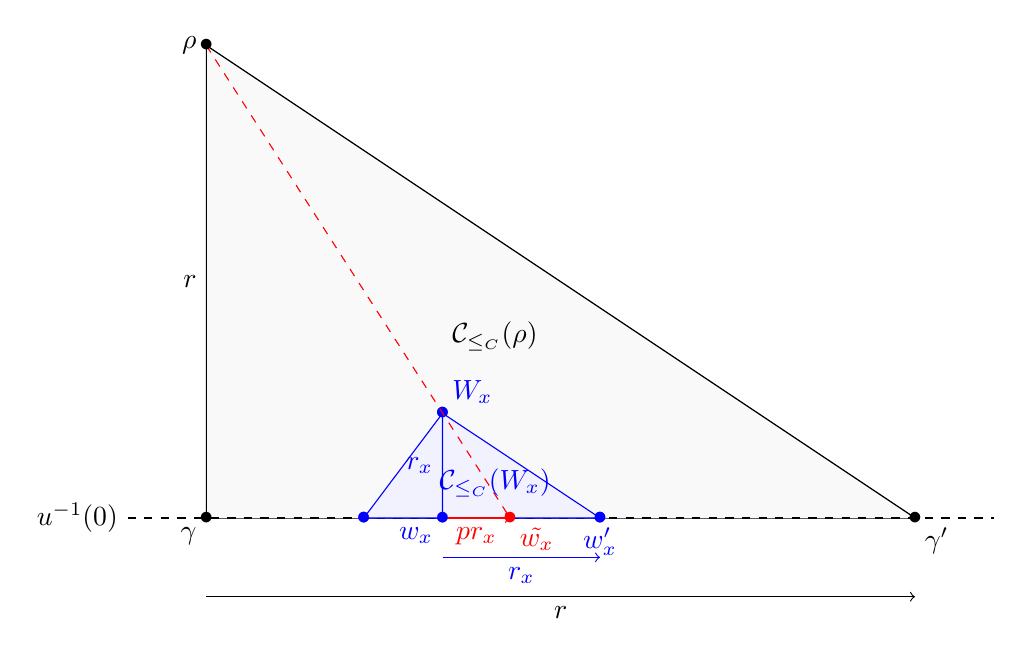
\begin{tikzpicture}
            \draw (0,0) coordinate (m) node [below left] {$\gamma$} -- (9,0) coordinate (m')  node [below right] {$\gamma'$} -- (0,6) coordinate (M)  node [left] {$\rho$};
            \draw (m) -- (M);
            \draw[draw,fill=gray!05] (m)--(M)--(m');
            \draw[dashed] ($($(m)-(1,0)$)$)  node[left] {$u^{-1}(0)$}  -- ($($(m')+(1,0)$)$);
            \draw[blue] ($1/3*($(m)+(m')$)$) coordinate (wi) node {$\bullet$} node [below left] {$w_x$};
            \draw[blue] ($($(wi)+(2,0)$)$) coordinate (w') node {$\bullet$} node [below] {$w'_x$};
            \draw[blue] ($($(wi)-(1,0)$)$) coordinate (w'') node {$\bullet$};
            \draw[blue] ($($(wi)+(0,1.33)$)$) coordinate (Wi) node {$\bullet$} node [above right] {$W_x$};
            \draw[blue, fill=blue!05] (wi) -- (Wi) -- (w') -- (w'') -- (Wi);
            \draw[red] ($($(wi)+(0.857,0)$)$) coordinate (wt) node {$\bullet$} node [below right] {$\tilde{w_x}$};
            \draw[red,->] (wi) -- (wt);
            \draw[red] (wt) ($1/2*($(wi)+(wt)$)$) node[below] {$pr_x$};
            \draw[blue] (wi) node {$\bullet$} (Wi) node {$\bullet$} (w') node {$\bullet$} (w'') node {$\bullet$};
            \draw[red, dashed] (M) -- (wt);
            \draw ($1/2*($(m)+(M)$)$) node[left] {$r$};
            \draw[blue] ($1/2*($(wi)+(Wi)$)$) node[left] {$r_x$};
            
            \draw[blue,->] ($($(wi)-(0,0.5)$)$) coordinate (a) -- ($($(w')-(0,0.5)$)$) coordinate (b);
            \draw[blue] ($1/2*($(a)+(b)$)$) node[below] {$r_x$};
            \draw[->] ($($(m)-(0,1)$)$) coordinate (c) -- ($($(m')-(0,1)$)$) coordinate (d);
            \draw ($1/2*($(c)+(d)$)$) node[below] {$r$};
            \draw (m) node {$\bullet$} (M) node {$\bullet$} (m') node {$\bullet$};
            \draw ($1/3*($(m)+(M)+(m')$)$) node[above right] {$\mathcal{C}_{\leq_C}(\rho)$};
            \draw[blue] ($1/3*($(wi)+(Wi)+(w')$)$) node {$\mathcal{C}_{\leq_C}(W_x)$};
          \end{tikzpicture}
        \end{center}
        \caption{Geometric visualization of points and gauge values defined in the proof of theorem \ref{theoEquivGen}}
      \end{figure}
      
      Let $\tilde{w_x} = w_x +\frac{r_x}{r-r_x}(w_x-\gamma) =\gamma+\frac{r}{r-r_x}(w_x-\gamma)$.   
      We show that $W_x = \rho+ \frac{r-r_x}{r}(\tilde{w_x}-\rho)$ and $\tilde{w_x} \in \mathcal{D}_{\Gamma}(\gamma,r)$, which means that $W_x \in \mathcal{C}_{\leq_C}(\rho)$ since $r_x \leq r$ by definition of $r$. First:
      
      \begin{equation}
        \begin{aligned}
          \rho+ \frac{r-r_x}{r}(\tilde{w_x}-\rho) &=\gamma+ rc + \frac{r-r_x}{r}(\gamma + \frac{r}{r-r_x}(w_x-\gamma) - (\gamma + rc))\\
          &=\gamma+(w_x-\gamma) + (r-(r-r_x))c = w_x + r_xc = W_x
        \end{aligned}
      \end{equation}
      
      
      Let us show now that $\tilde{w_x} \in \mathcal{D}_{\Gamma}(\gamma,r)$. Let us call the following unit gauge direction $\vec{u} := \frac{w_x-\gamma}{\norm{w_x-\gamma}_{\Gamma}}$. Let $w'_x$ be the point at the border of $\mathcal{D}_{\Gamma}(w_x,r_x)$ in the direction $\vec{u}$ going from $w_x$: $w'_x= w_x + r_x\vec{u} \in \mathcal{D}_{\Gamma}(w_x,r_x)$. For all $p \in [0,1]$ we have by convexity of $\mathcal{D}_{\Gamma}(w_x,r_x)$ that $w_p = pw'_x + (1-p)w_x = w_x+pr_x\vec{u} \in \mathcal{D}_{\Gamma}(w_x,r_x) \subseteq \mathcal{D}_{\Gamma}(\gamma,r)$. But:
      
      \[ \tilde{w_x} = w_x + \frac{r_x}{r-r_x}(w_x-\gamma) = w_x + \frac{\norm{w_x-\gamma}_{\Gamma}}{(r-r_x)}r_x\vec{u} = w_{\frac{\norm{w_x-\gamma}_{\Gamma}}{(r-r_x)}} \]
      
      So we have only to prove that $\norm{w_x-\gamma}_{\Gamma} \leq r-r_x$ to get that $\tilde{w_x} \in \mathcal{D}_{\Gamma}(w_x,r_x) \subseteq \mathcal{D}_{\Gamma}(\gamma,r)$.
      
      Let $\gamma'$ be the point at the border of $\mathcal{D}_{\Gamma}(\gamma,r)$ in the direction $\vec{u}$ going from $\gamma$. Then $\gamma' = \gamma+r\vec{u}$. Also, $w_x' = w_x + r_x\vec{u} = \gamma + (r_x+\norm{w_x-\gamma}_{\Gamma})\vec{u}$ is in the direction $\vec{u}$ going from $\gamma$. Since $w_x' \in \mathcal{D}_{\Gamma}(w_x,r_x) \subseteq \mathcal{D}_{\Gamma}(\gamma,r)$ and $\gamma'$ is at the border of $\mathcal{D}_{\Gamma}(\gamma,r)$ in the same direction $\vec{u}$ from the same point $\gamma$, we have that $\norm{w_x' - \gamma}_{\Gamma} \leq \norm{\gamma'-\gamma}_{\Gamma}$ so $r_x+\norm{w_x-\gamma}_{\Gamma} \leq r$ ie. $\norm{w_x-\gamma}_{\Gamma} \leq r-r_x$.
      
      Thus $W_x \leq_C \rho$, and this is true for all $x \in S$, so $\rho$ is a feasible solution of MinEffect$^*$.
    \end{enumerate}
  \end{proof}
  
  \begin{cor}
    MECP$^*$ and MinEffect$^*$ are equivalent problems.
  \end{cor}
  
  \begin{proof}
    Both problems have the same feasible solutions thanks to theorem \ref{theoEquivGen}, and the parameter we minimize is the same in both case, so optimal solutions from one problem map to optimal solutions of the other problem.
  \end{proof}
\end{subsubsection}

\begin{subsection}{Useful properties of MECP from \cite{BK13,BR09}}
  Here we assume here that $P$ in MECP is only compact and not finite. We have the following results:
  \begin{theo}[Optimality conditions]
    \label{optCond}
    $P$ is optimally contained in $\Gamma$ iff:
    \begin{enumerate}
    \item $P \subseteq \Gamma$
    \item For some $2 \leq k \leq n + 1$, there exist $p_1, \ldots , p_k \in P$ and hyperplanes $H(a_i,1)$ supporting $P$ and $\Gamma$ in $p_i$ s.t. $0  \in \text{conv}\set{a_1,\ldots,a_k}$.
    \end{enumerate}
  \end{theo}
  
  \begin{figure}[!h]
    \begin{center}
      \includegraphics[scale=0.2]{optCond.png}
    \end{center}
    \caption{Illustration of optimality conditions (Theorem \ref{optCond})}
  \end{figure}

  \begin{defi}[Core-radii]
    The \emph{$k$-th core-radius} of $P$ with respect to $\Gamma$ is defined by:
    \[ R_k(P,\Gamma) := \underset{S \subseteq P, \abs{S} \leq k+1}{\max} R(S,\Gamma) \]
    In particular: $S(W,k) = \frac{1}{k}(1 + R_{k-1}(W-c,-\Omega_c))$
  \end{defi}
  \begin{figure}[!h]
  \begin{multicols}{2}
    \begin{center}
      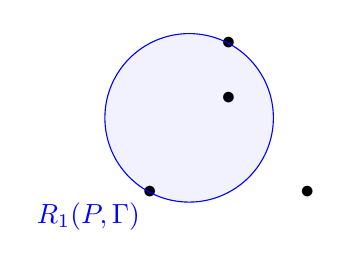
\begin{tikzpicture}
        \draw (0,0) coordinate (A) node {$\bullet$} (2,0) coordinate (B) node {$\bullet$}  (1,1.9) coordinate (C) node {$\bullet$};
        \draw (1,1.2) coordinate (D) node {$\bullet$};
        \draw[darkgreen] ($1/2*($(A)+(C)$)$) coordinate (G);
        \draw[blue,fill,fill opacity=0.05] (G) circle (1.07); 
        \draw[blue] (A) node[below left] {$R_1(P,\Gamma)$};
      \end{tikzpicture}
    \end{center}

    \columnbreak
    
      \begin{center}
        \begin{tikzpicture}
          \draw (0,0) coordinate (A) node {$\bullet$} (2,0) coordinate (B) node {$\bullet$} (1,1.9) coordinate (C) node {$\bullet$};
          \draw (1,1.2) coordinate (D) node {$\bullet$};
          \draw[blue,fill,fill opacity=0.05] (G) circle (1.07); 
          \draw[red,fill,fill opacity=0.05] (1,0.69) circle (1.22);
          \draw[red] (B) node[right] {$R_2(P,\Gamma)$};
        \end{tikzpicture}
      \end{center}
  \end{multicols}
  \caption{Illustration of several core-radii}
  \end{figure}

  \begin{theo}[Helly's theorem]
    If $\dim(P) \leq k$, then $R_k(P,\Gamma) = R(P,\Gamma)$. \underline{For us:} $\dim(V)+1$ measurement outputs used at most.
  \end{theo}
  
  \begin{theo}[$R_k/k$ decreases]
    \[\Big(\frac{R_k(P,\Gamma)}{k}\Big)_{k \in [n]} \text{ decreases. \underline{For us:} } \Big(\frac{S(W,k) - \frac{1}{k}}{1 - \frac{1}{k}}\Big)_{k \in [n]} \text{ decreases.}\]
  \end{theo}

  \begin{prop}
    Let $\varphi(\gamma) := \min\set{r:P \subseteq r\Gamma}$ defined on $\mathbb{R}^n$. Then $\varphi$ is convex, and in particular it has subgradients.
  \end{prop}

  \begin{proof}
    Let $x,y \in \mathbb{R}^n$ and $\lambda \in [0,1]$. Let us show that:
    \[\varphi(\lambda x + (1-\lambda)y) \leq \lambda \varphi(x) + (1-\lambda)\varphi(y)\]

    For this we will use the following lemma on convex sets:
    \begin{lem}
        If $C$ is a convex set and $a,b>0$, then $aC+bC=(a+b)C$.
      \label{lemConvSet}
    \end{lem}

    \begin{proof}
      $aC+bC\supseteq(a+b)C$ is immediate and always true. If $x \in aC+bC$, there exists $y,z \in C$ such that $x = ay+bz=(a+b)w$ where:
      \[w =  \frac{a}{a+b}y+\frac{b}{a+b}z \in C\]
      since $C$ is convex and $\frac{a}{a+b}+\frac{b}{a+b}=1$.
    \end{proof}

    Then by definition of $\varphi$, we have that $P \subseteq C_x := x + \varphi(x)\Gamma$ and $P \subseteq C_y := y + \varphi(y)\Gamma$, so $P \subseteq \lambda C_x + (1-\lambda) C_y$. Since $C_x$ and $C_y$ are convex, by lemma \ref{lemConvSet}, we have that:
    \begin{equation}
      \begin{aligned}
        P \subseteq \lambda C_x + (1-\lambda) C_y &=& \lambda x + (1-\lambda)y +  \lambda\varphi(x)C + (1-\lambda)\varphi(y)C \\
        &=& \lambda x + (1-\lambda)y +  (\lambda\varphi(x) + (1-\lambda)\varphi(y))C
      \end{aligned}
    \end{equation}
    But since $\varphi(\lambda x + (1-\lambda)y)$ is the minimum dilation coefficient of such an inclusion, we have that $\varphi(\lambda x + (1-\lambda)y) \leq \lambda \varphi(x) + (1-\lambda)\varphi(y)$.
  \end{proof}

  \begin{prop}
    If $a$ is a subgradient of $\varphi$ at $c$ then $-a$ is an outer normal of a hyperplane supporting $c + \varphi(c)\Gamma \supseteq P$ at $p_i \in P$.
  \end{prop}

  \begin{defi}[Core-set]
    $S \subseteq P$ is a $\epsilon$-\emph{core-set} of P if $R(S,\Gamma) \leq R(P,\Gamma) \leq (1+\epsilon)R(S,\Gamma)$\\
  \end{defi}

  \begin{theo}
    For all $P,\Gamma \subseteq \mathbb{R}^n, \epsilon \geq 0$, there exists an $\epsilon$-core-set of size at most $\lceil\frac{n}{1+\epsilon}\rceil+1$.\\
    Moreover, for any $\epsilon < 1$ there exist $P \subseteq \mathbb{R}^n$ and a $0$-symmetric convex body $\Gamma$ (ie. $\Gamma = -\Gamma$) such that no smaller subset of $P$ suffices.\\
    Also, this bound is optimal for the $n$-regular simplex.
  \end{theo}

  \begin{rk}
    The MEC of some set of points is not necessarely unique, for instance it isn't for squares. However, in the shapes we will study, we will look at the cases where it is unique.
  \end{rk}
\end{subsection}

\begin{subsection}{Geometric interpretation}
  \begin{subsubsection}{Simplex: classical case}
    When the shape $\Gamma$ is the opposite of the probability simplex $\Omega_c = T^n := \set{x \in \mathbb{R_+}^{n+1} : u(x) := \sum_{i = 1}^{n+1} x_i = 1}$, it corresponds to the classical problem of channel coding. Up to an affine transformation, we get in this way all classical cones. For them, the function $f_W$ is submodular (since $f_W$ is submodular for the probability simplex and MECP is stable by affine transformations). In particular we have some basic interpretation of submodularity in the shapes:
    \begin{prop}
      If $f_W$ is submodular, then MEC$(S) \subseteq$ MEC$(T)$ for $S \subseteq T$ if MEC is unique.
    \end{prop}

    \begin{proof}
      By contraposition. Let $S \subset T$ such that MEC$(S) \not\subseteq$ MEC$(T)$. There exists thus $x$ such that $x \in$ MEC$(S)$ and $x \not\in$ MEC$(T)$, so in particular $x \not\in T$. This implies that MEC$(S\cup\set{x}) =$ MEC$(S)$, so $f_w(S\cup\set{x}) = f_W(S)$, but MEC$(T) \not\subseteq$ MEC$(T\cup\set{x})$, so by unicity of MEC and monocity of $f_w$ that $f_w(T\cup\set{x}) > f_W(T)$, so $f_w$ is not submodular.
    \end{proof}

    We conjecture that this property is in fact an equivalence, and is fulfilled only for simplices, where MEC ar unique as a consequence of the uniqueness of the supremum $\rho$ in that cone.

    \begin{center}
        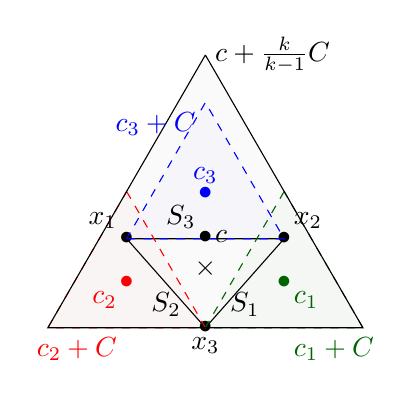
\begin{tikzpicture}
          \draw (0,0) coordinate (A) node {$\bullet$} node[above left] {$x_1$} -- (2,0) coordinate (B) node {$\bullet$}  node[above right] {$x_2$} -- (1,-1.13) coordinate (C) node {$\bullet$}  node[below] {$x_3$} -- (A);
          \draw ($1/2*($(A)+(B)$)$) node[above left] {$S_3$};
          \draw ($1/2*($(A)+(C)$)$) node[below] {$S_2$};
          \draw ($1/2*($(B)+(C)$)$) node[below] {$S_1$};
          \draw[dashed, blue, fill,fill opacity=0.02] (A)--(B)--(1,1.73) coordinate (D)--(A);
          \draw[dashed, red, fill,fill opacity=0.02] ($(A)+(0,0.6)$)--(C)--($(-1,-1.73)+(0,0.6)$) coordinate (E)--($(A)+(0,0.6)$);
          \draw[dashed, darkgreen, fill,fill opacity=0.02] ($(B)+(0,0.6)$)--(C)--($(3,-1.73)+(0,0.6)$) coordinate (F)--($(B)+(0,0.6)$);
          \draw[darkgreen] ($1/3*($($(B)+(0,0.6)$)+(C)+(F)$)$) coordinate (c1) node {$\bullet$} node[below right] {$c_1$};
          \draw[red] ($1/3*($($(A)+(0,0.6)$)
          +(C)+(E)$)$) coordinate (c2) node {$\bullet$} node[below left] {$c_2$};
          \draw[blue] ($1/3*($(A)+(B)+(D)$)$) coordinate (c3)  node {$\bullet$} node[above] {$c_3$};
          \draw ($1/3*($(A)+(B)+(C)$)$) coordinate(0) node {$\times$};
          \draw ($1/3*($(c1)+(c2)+(c3)$)$) coordinate (c0);
          \draw ($(c0)+($($(c0)-(0)$)$)$) coordinate (c) node {$\bullet$} node[right] {$c$};
          \draw ($(c)+(0,2.31)$) coordinate (X) node[right] {$c+\frac{k}{k-1}C$};
          \draw[fill,fill opacity=0.02] (X)--(E)--(F)--(X);
          \draw[darkgreen] ($1/2*($(C)+(F)$)$) node[below right] {$c_1+C$};
          \draw[red] ($1/2*($(C)+(E)$)$) node[below left] {$c_2+C$};
          \draw[blue] (D) node[below left] {$c_3+C$};
        \end{tikzpicture}
    \end{center}
    
  \end{subsubsection}
  \begin{subsubsection}{$\mathcal{D}_d$: quantum case}
    Let us call $\mathcal{D}_d := \set{M \in \mathcal{H}_d : M \succcurlyeq 0 \text{ and } \Tr(M) = 1}$ the set of quantum states. In the quantum context, we take for convenience $c = \mathbbm{1}_d := \frac{1}{d}\mathbbm{1}$, and we call $Q_d := \Omega_c = \mathcal{D}_d - \mathbbm{1}_d$. The equivalent MEC problem is given by $P = W - \mathbbm{1}_d \subseteq Q_d$ and $\Gamma := - \Omega_c = -Q_d$
    \paragraph{Qubit case ($d = 2$):}
    \label{geoQubit}
    Here we have that $Q_2$ is isometric to the Bloch sphere $\mathbb{B}_3$ and $P$ are the coordinates of $W$ in that sphere. We have in particular that $Q_2$ is symmetric, ie. $Q_2=-Q_2 = \Gamma$. Thus we are reduced to find the Minimum Enclosing Ball of points (which will be discussed more generally in section \ref{balls}) to compute one value of MECP.
    This interpretation was found by \cite{DT10} in the dimension $2$ case, with some interpretation of non-uniform inputs which we can also interpret with our problem MECP$^*$ as a Minimum Enclosing Ball of Balls problem, first studied by \cite{Megiddo89}. In both cases, these can be computed efficiently without using SDPs.

    In particular, for pure qubit states, we can now prove the following corollary:
    \begin{cor}
      In the real, pure and dimension 2 case, we have the following property for a set of states $\set{W_x = \dyad{\psi_x}}_{x \in S}$. Let $\theta_S$ be the minimum angle such that all states of $S$ can be put in a slice of the Bloch circle of radius $\theta$. Then $f_W(S) = g(\theta_S)$ where:
      \[
      g(\theta)=\begin{cases}
      1 + \sin(\frac{\theta}{2}) \text{ if } 0 \leq \theta \leq \pi\\
      2 \text{ if } \pi \leq \theta \leq 2\pi
      \end{cases}
      \]
      \label{corPureReal}
      \end{cor}

    \begin{proof}
      If all states are in one hemisphere of the Bloch circle, the minium enclosing circles of all states is the minimum enclosing circle of extremal ones (depicted as $W_1$ and $W_k$ in the drawing below).
      \begin{center}
        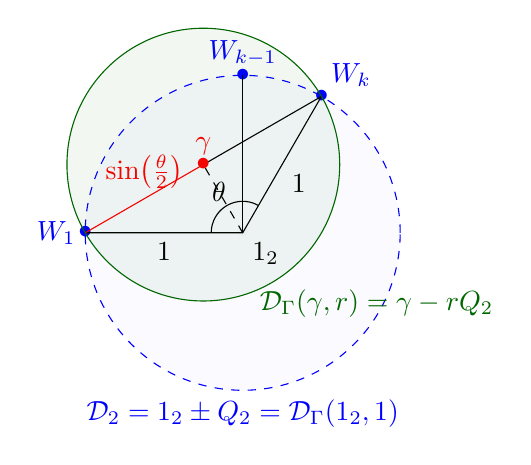
\begin{tikzpicture}
          \draw[dashed,blue,fill, fill opacity = 0.02] (0,0) coordinate (O) node {$\bullet$} circle (2);
          \draw[blue] (0,-2) node[below] {$\mathcal{D}_2 = \mathbbm{1}_2 \pm Q_2 = \mathcal{D}_{\Gamma}(\mathbbm{1}_2,1)$};
          \draw (O) node[below right] {$\mathbbm{1}_2$};
          \draw[blue] (-2,0) coordinate (A) node {$\bullet$};
          \draw[blue] (A) node[left] {$W_1$};
          \draw[dashed,blue] (0,2) coordinate (B) node {$\bullet$};
          \draw[blue] (B) node[above] {$W_{k-1}$};
          \draw[blue] (1,1.732) coordinate (C) node {$\bullet$};
          \draw[blue] (C) node[above right] {$W_k$};
          \draw (A) -- (O) -- (C);
          \draw (O) -- (B);
          \draw pic["$\theta$", draw=black, angle eccentricity=1.5, angle radius=0.4cm] {angle=C--O--A};
          \coordinate (D) at ($0.5*($(A)+(C)$)$);
          \draw (D) -- (C);
          \draw[dashed] (O) -- (D);
          \draw[red] (A) -- (D);
          \draw[red] ($0.5*($(A)+(D)$)$) node[above] {$\sin(\frac{\theta}{2})$};
          \draw[red] (D) node {$\bullet$};
          \draw[red] (D) node[above] {$\gamma$};
          \draw ($0.5*($(A)+(O)$)$) node[below] {$1$};
          \draw ($0.5*($(C)+(O)$)$) node[below right] {$1$};
          \draw[darkgreen,fill, fill opacity = 0.05] (D) circle (1.732);
          \draw[darkgreen] (1.7,-0.9) node {$\mathcal{D}_{\Gamma}(\gamma,r) = \gamma - rQ_2$};
        \end{tikzpicture}
      \end{center}

      Then, by a simple use of Pythagore, we get that the radius of that circle is given by $r =\sin(\frac{\theta}{2})$, so $f_W(S)= 1 + \sin(\frac{\theta_S}{2}) = g(\theta_S)$ for $0 \leq \theta_S \leq \pi$.

      Otherwise, if we can't put allo states in one hemisphere, by optimality conditions of MECP, we get that $\mathcal{D}_{\Gamma}(\mathbbm{1}_2,1)$ is optimal, so that $r=1$, ie. $f_W(S)= 2 = g(\theta_S)$ for $\theta_S \geq \pi$.
      \end{proof}
    
    \paragraph{General case:}
      \begin{itemize}
      \item We look at $Q_d = \mathcal{D}_d-\mathbbm{1}_d \subseteq \mathbbm{R}^n$ with $n=d^2-1$ which is not symmetric as soon as $d>2$.
      \item MEQ of a set of points is unique since the dual quantum channel coding problem has a unique solution.
      \item In $\Gamma$: $0$ is equidistant from all extremal points (pure states).
      \item $\mathcal{B}\Big(0,\frac{1}{\sqrt{d(d-1)}}\Big) \subseteq \Gamma \subseteq \mathcal{B}\Big(0,\sqrt{1-\frac{1}{d}}\Big)$ and tight ratio $d-1$.
      \item Like $T^{d-1}$, no $\epsilon$-core-sets of size $< \lceil\frac{d-1}{1+\epsilon}\rceil + 1$:
      if $k < \lceil\frac{d-1}{1+\epsilon}\rceil$, then for $\abs{S} \leq k+1$: 
      $R(\mathcal{D}_d,-Q_d)=\frac{d-1}{k}R_k(\mathcal{D}_d,-Q_d) > (1+\epsilon)R_k(\mathcal{D}_d,-Q_d) \geq (1+\epsilon)R(S,-Q_d)$
      \end{itemize}
  \end{subsubsection}
  \begin{subsubsection}{Ball $\mathbb{B}_n$}
    \label{balls}
    We study here the case of MECP where we have $\Gamma := \mathbb{B}_n$ is a $2-$norm ball in dimension $d$, which is a symmetric convex body. It is a well-studied problem, and a specific instance of MEBP can be computed efficiently (via an FPTAS), thanks to an algorithm by \cite{BK03} for instance. We can speak of the MEB of a set of points since it is unique for that shape.

    \paragraph{Efficient approximation}
    In the case of balls, optimality conditions can be rewritten in the following form:
    \begin{lem}[Half-space lemma]
      MEB$(P)$ is the minimum enclosing ball of $P \subseteq \mathbb{R}^n$ iff any closed half-space that contains the center $c_{\mathcal{B}(P)}$ also contains a point of $P$ on the boundary of MEB$(P)$.
  \end{lem}
    We have not yet been able to prove the efficiency of the generic greedy algorithm, but we hav another algorithm wich will efficiently approximate $S(W,k)$ via the existence of $\epsilon$-core-sets of size independent to the dimension in the case of balls:

    \begin{theo}[\cite{BK03}]
      \label{coreprop}
      An $\epsilon$-core-set $S_{\epsilon}$ of $P \subseteq \mathbb{R}^n$ of size $\lceil\frac{2}{\epsilon}\rceil$ can be efficiently computed. In particular, this gives a $(1+\frac{2}{k})$-approximation of $R_k(P,C)$.
    \end{theo}
  
  \begin{proof}[Proof of Corollary]
    Let $\epsilon$ such that $k+1 = \lceil\frac{2}{\epsilon}\rceil = \abs{S_{\epsilon}}$. Then $\epsilon \leq \frac{2}{k}$, so $R_k(P,\Gamma) \leq R(P,\Gamma) \leq (1+\epsilon)R(S_{\epsilon},\Gamma) \leq (1+\frac{2}{k})R(S_{\epsilon},\Gamma)$.
  \end{proof}

  \begin{rk}
    This decreasing approximation ratio gives in particular the existence of a PTAS computing $R_k(P,\Gamma)$ (and so $S(W,k)$):
    
    Let $\epsilon > 0$ fixed.
    \begin{itemize}
    \item If $\epsilon \geq \frac{2}{k}$, then we run the previous algorithm which gives a $(1 + \frac{2}{k})$-approximation, so in particular a $(1 + \epsilon)$-approximation.
    \item If $\epsilon < \frac{2}{k}$, then $k < \frac{2}{\epsilon}$ is bounded by a constant, so we do an exhaustive search of all sets of size $k$, which will be done in time $\mathcal{O}(\abs{P}^{\frac{2}{\epsilon}})$ which is polynomial.
    \end{itemize}
    
  \end{rk}
  To get such a core-set we wil use the following algorithm.
  
  \begin{algorithm}[H]
      \DontPrintSemicolon
      
      \KwInput{$k \in \set{1, \ldots, \abs{P}}$}
      \KwOutput{An $\frac{2}{k}$-core-set $S_k$ of $P \subseteq \mathbb{R}^n$ of size $k+1$}
      $S_0 = \set{p}$ with $p$ any point of $P$\\
      $c_0 = p, r_0 = 0$ \tcp*{Center and radius of MEB of $S_0$}
      \For{$i \in \set{1,\ldots,k}$}
         {
           $q_i =$ furthest point from $c_{i-1}$ in $P$\\
           $S_{i} = S_{i-1} \cup \set{q_i}$\\
           $c_i,r_i$ such that MEB($S_i)=\mathcal{B}(c_i,r_i)$\\
         }
         
         \Return $S_k$
         \caption{Ball algorithm \cite{BK03}}
         \label{ballAlgo}
  \end{algorithm}

  We show now some example where the greedy choice is different from the generic greedy algorithm:

  \begin{figure}[!h]
    \begin{multicols}{2}
      \begin{center}
        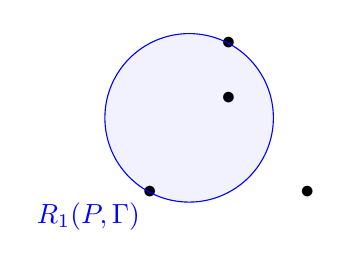
\begin{tikzpicture}
          \draw (0,0) coordinate (A) node {$\bullet$} (2,0) coordinate (B) node {$\bullet$}  (1,1.9) coordinate (C) node {$\bullet$};
          \draw (1,1.2) coordinate (D) node {$\bullet$};
          \draw[darkgreen] ($1/2*($(A)+(C)$)$) coordinate (G);
          \draw[blue,fill,fill opacity=0.05] (G) circle (1.07); 
          \draw[blue] (A) node[below left] {$R_1(P,\Gamma)$};
        \end{tikzpicture}
      \end{center}

      \columnbreak
      
      \begin{center}
        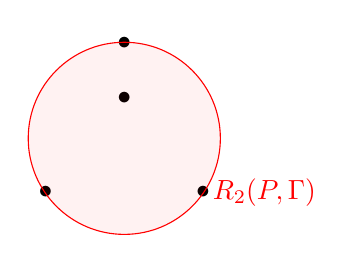
\begin{tikzpicture}
          \draw (0,0) coordinate (A) node {$\bullet$} (2,0) coordinate (B) node {$\bullet$} (1,1.9) coordinate (C) node {$\bullet$};
          \draw (1,1.2) coordinate (D) node {$\bullet$};
          \draw[red,fill,fill opacity=0.05] (1,0.69) circle (1.22);
          \draw[red] (B) node[right] {$R_2(P,\Gamma)$};
        \end{tikzpicture}
      \end{center}
    \end{multicols}
    \begin{multicols}{3}
      \begin{center}
        \begin{tikzpicture}
          \draw (0,0) coordinate (A) node {$\bullet$} node[below left] {$2$} (2,0) coordinate (B) node {$\bullet$}  node[below right] {$3$} (1,1.9) coordinate (C) node {$\bullet$} node[right] {$4$};
          \draw (1,1.2) coordinate (D) node {$\bullet$} node[left] {$1$};
          \draw[blue,fill,fill opacity=0.05] (G) circle (1.07);
          \draw[darkgreen,dashed] (A)--(D)--(C) (D)--(B);
          \draw[darkgreen] ($1/2*($(A)+(D)$)$) coordinate (E) node {$\bullet$} node[right] {$c_1$};
          \draw[darkgreen,fill,fill opacity=0.05] (E) circle (0.79);
          \draw[darkgreen] (-0.6,0.3) node {$S_1$};
        \end{tikzpicture}
      \end{center}
      
      \columnbreak
      
      \begin{center}
        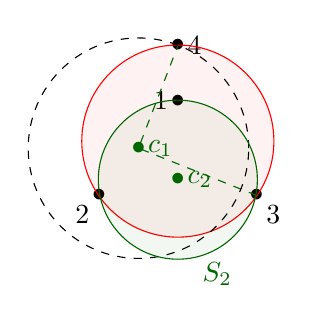
\begin{tikzpicture}
          \draw (0,0) coordinate (A) node {$\bullet$} node[below left] {$2$} (2,0) coordinate (B) node {$\bullet$}  node[below right] {$3$} (1,1.9) coordinate (C) node {$\bullet$} node[right] {$4$};
          \draw (1,1.2) coordinate (D) node {$\bullet$} node[left] {$1$};
          \draw[red,fill,fill opacity=0.05] (1,0.69) circle (1.22);
          \draw[darkgreen] ($1/2*($(A)+(D)$)$) coordinate (E) node {$\bullet$} node[right] {$c_1$};
          \draw[darkgreen,dashed] (B)--(E)--(C);
          \draw[dashed] (E) circle (1.4);
          \draw[darkgreen] (1,0.2) coordinate (F) node {$\bullet$} node[right] {$c_2$};
          \draw[darkgreen,fill,fill opacity=0.05] (F) circle (1.01);      
          \draw[darkgreen] (1.5,-1) node {$S_2$};
        \end{tikzpicture}
      \end{center}

      \columnbreak
      
      \begin{center}
        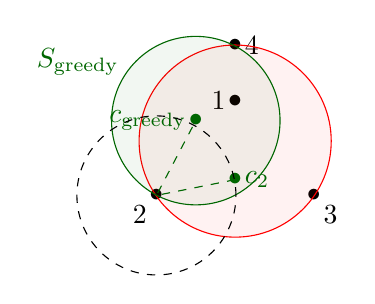
\begin{tikzpicture}
          \draw (0,0) coordinate (A) node {$\bullet$} node[below left] {$2$} (2,0) coordinate (B) node {$\bullet$}  node[below right] {$3$} (1,1.9) coordinate (C) node {$\bullet$} node[right] {$4$};
          \draw (1,1.2) coordinate (D) node {$\bullet$} node[left] {$1$};
          \draw[red,fill,fill opacity=0.05] (1,0.69) circle (1.22);
          \draw[darkgreen] (1,0.2) coordinate (F) node {$\bullet$} node[right] {$c_2$};
          \draw[darkgreen] ($1/2*($(A)+(C)$)$) coordinate (G) node {$\bullet$} node[left] {$c_{\text{greedy}}$};
          \draw[darkgreen,dashed] (F)--(A)--(G);
          \draw[darkgreen,fill,fill opacity=0.05] (G) circle (1.07);
          \draw[darkgreen] (-1,1.7) node {$S_{\text{greedy}}$};
          \draw[dashed] (A) circle (1.01);
        \end{tikzpicture}
      \end{center}
    \end{multicols}
    \caption{Differences between algorithms \ref{greedy} and \ref{ballAlgo}}
  \end{figure}

  \begin{proof}[Proof sketch of Theorem \ref{coreprop}, done in \cite{BK03}]
    If at some point $c_{i+1} = c_i$, then we have an MEB of all $P$, so it will be in particular a $\epsilon$-core-set. We assume this never happens. At step $i$, take $H \ni c_i$ with $H \perp \overset{\rightarrow}{c_ic}_{i+1}$, and $p \in \partial\mathcal{B}(S_i) \cap H^+ \cap S_i$ thanks to the half-space lemma. By geometric arguments, we get two inequalities:
    \begin{enumerate}
      \item $r_{i+1} \geq \norm{c_{i+1}-p}_2 \geq \sqrt{r_i^2+\norm{c_{i+1}-c_i}_2^2}$ by Pythagore.
      \item $r_{i+1} \geq \norm{c_{i+1}-q_{i+1}}_2 \geq R - \norm{c_{i+1}-c_i}_2$ since $q_{i+1}$ furthest point away from $c_i$.
    \end{enumerate}
    
    This will imply by studying the worst case in this inequality, $\sqrt{r_i^2+\norm{c_{i+1}-c_i}_2^2} = R - \norm{c_{i+1}-c_i}_2$, that after $k = \lceil\frac{2}{\epsilon}\rceil$ steps, we get $R \leq (1+\epsilon)r_k$.
  \end{proof}
  
  \paragraph{NP-hardness and inapproximability result}
  \begin{description}
  \item[\underline{Problem:}] \emph{BallChannelCoding}
  \item[\underline{Instance:}] A finite set $P \subseteq \mathbb{R}^d$ of points of size $n$, $R \in \mathbb{R}$ and $k \in \set{1,\ldots,n}$
  \item[\underline{Question:}] Does $R_{k-1}(P,\Gamma) (=kS(W,k)-1) \geq R$, where $\Gamma = \mathbb{B}^d$ ?
  \end{description}

  \begin{theo}
    \label{theoBallChannelCoding}
    \emph{BallChannelCoding} is NP-hard. Furthermore, its optimization version is even NP-hard to approximate within a factor $1 - \frac{1}{4k^2} + \epsilon$ for $\epsilon > 0$. In particular, there does not exist a FPTAS that solves this problem if $P \not= NP$.
  \end{theo}

  In order to prove this theorem, we will need some lemmas on the MEB of points:

  \begin{lem}
    \label{lemball}
    \begin{enumerate}
      \item The center $c$ of the MEB of $P$ lies in the convex hull of $P$.
      \item If a point $c$ is equidistant from all points in $P$ and $c$ lies in the convex hull of $P$, then $c$ is the center of the MEB of $P$ and its radius is given by $\norm{p-c}_2$ for any $p \in P$.
    \end{enumerate}
  \end{lem}

  \begin{proof}
    \begin{enumerate}
      \item This is a consequence of the half-space lemma: if $c$ is outside the convex hull of $P$, there exist a hyperplan $H \ni c$ such that $P$ is included in the one of the open half-spaces induced by $H$, which is in contradiction with the half-space lemma.
      \item We use the fact that $a \in$ CH$(P) \iff \forall u : \norm{u}_2 = 1, \min_{p \in P} (p-a)^Tu \leq 0$.

        We first remark that $\mathbb{B}(c,d)$, where $d = \norm{c-p}_2$ for $p \in P$ is an enclosing ball of $P$ since $c$ is equidistant from $P$. Let us assume by contradiction that it is not the MEB of $P$, but that MEB$(P) = \mathbb{B}(c',d')$. We have $d' < d$ since otherwise $\mathbb{B}(c,d)$ is the MEB of $P$. Thus this implies that $c'\not=c$ since $p \not\in \mathbb{B}(c,d')$ for $p \in P$ since  $\norm{c-p}_2 = d > d'$.

        Let us define $u = \frac{c'-c}{\norm{c'-c}_2}$. Since $c \in$ CH$(P)$, we have that $\min_{p \in P} (p-c)^Tu \leq 0$, so there exists some $p \in P$ such that $(p-c)^Tu \leq 0$. Thus:
        \begin{equation}
          \begin{aligned}
            \norm{p-c'}_2 &=&& \norm{p-c+c-c'}_2 = \sqrt{\norm{p-c}_2^2 +\norm{c-c'}_2^2 + 2(p-c)^T(c-c')}\\
            &=&& \sqrt{d^2 +\norm{c-c'}_2^2 - 2\norm{c-c'}_2(p-c)^Tu} \geq \sqrt{d^2 +\norm{c-c'}_2^2} > d
          \end{aligned}
        \end{equation}
        since $(p-c)^Tu \leq 0$, which leads to a contradiction since $\norm{p-c'}_2 \leq d' < d$.
    \end{enumerate}
  \end{proof}

  
  \begin{proof}[Proof of Theorem \ref{theoBallChannelCoding}]
    Like for \emph{PureRealChannelCoding}, we will show that \emph{BallChannelCoding} is NP-complete with a reduction from \emph{X3C} define in section \ref{X3C}. We 

    We use the following reduction. Let $Q = \set{q_1,\ldots,q_m}$ and $C = \set{c_1,\ldots,c_n}$.
    We take $k=\floor{\frac{m}{3}}$, $R=\sqrt{1 - \frac{1}{k}}$, and $P =\set{p^j}_{j \in [n]} \subseteq \mathbb{R}^m$, where

    \[p^j_i = \begin{cases}
      \frac{1}{\sqrt{3}} \text{ if } q_i \in c_j\\
      0 \text{ otherwise}\\
    \end{cases}
    \]

    This is a valid instance of \emph{BallChannelCoding}.

    Let us show that there exists an exact cover for $Q$ if and only if $R_{k-1}(P,\Gamma) \geq R$.

    \begin{itemize}
    \item[$(\Rightarrow)$] If there is and exact cover $S$ of $Q$, then $\abs{S} = \frac{m}{3} \in \mathbb{N}$. We have then $\abs{S} = k$. We show that the MEB of $P_S := \set{p^j}_{j \in S}$ has a radius equals to $R=\sqrt{1 - \frac{1}{k}}$, which is enough to show that $R_{k-1}(P,\Gamma) \geq R$.

      Since $S$ is an exact cover of $Q$, this means that in $P_s$, each coordinate of all points is non-zero exactly once for some point where it is equal to $\frac{1}{\sqrt{3}}$. We have then that their barycenter $c_{\text{opt}} := \frac{1}{k}\pmqty{\frac{1}{\sqrt{3}}\\\vdots\\\frac{1}{\sqrt{3}}}$ is the center of the MEB, since it lies in their convex hull and it is equidistant from all of them, thanks to lemma \ref{lemball}. In that case, all points of $P_S$ are equidistant to the center $c_{\text{opt}}$, so the radius of the MEB is given by:
      \begin{equation}
        \begin{aligned}
          r_{P_S} &=&& \norm{p^{s_1}-c_{\text{opt}}}_2 = \sqrt{3\times\Big(\frac{1}{\sqrt{3}}\Big(1-\frac{1}{k}\Big)\Big)^2 + (m-3)\times\Big(\frac{1}{k\sqrt{3}}\Big)^2} \\
          &=&&\sqrt{\Big(1-\frac{1}{k}\Big)^2 + \frac{m}{3k^2} - \frac{1}{k^2}} = \sqrt{\Big(1 - \frac{2}{k} + \frac{1}{k^2}\Big) + \frac{1}{k} - \frac{1}{k^2}} \\
          &=&& \sqrt{1 - \frac{1}{k}} = R
        \end{aligned}
      \end{equation}
      
    \item[$(\Leftarrow)$] We first remark that in the previous situation, the MEB of $P_S$ which we call $\mathbb{B}(c_{\text{opt}},R)$ is in fact enclosing all the points possible coming from a reduction from \emph{X3C}. Thus $R$ is the maximal value that can be achieved.

      We show this by contradiction. We assume that there does not exist any exact cover for $Q$. Thus for any set $T$ of size $k$, there is a least one coordinate which is not covered by any points of $P_T$ since $3k \leq m$, so all coordinates are covered if and only if we have an exact cover. Thus their MEB is different from the previous one $\mathbb{B}(c_{\text{opt}},R)$, since its center lies in a subspace which does not contain $c_{\text{opt}}$ thanks to lemma \ref{lemball}. By unicity of MEBs, this implies that the radius of the MEB of $P_T$ is strictly smaller than the radius of $\mathbb{B}(c_{\text{opt}},R)$, since it is also an enclosing ball of our current instance. Thus we get that $r_{P_S} < R$, ie.  $R_{k-1}(P,\Gamma) < R$ since it is true for any set $T$ of size $k$.
      
    \end{itemize}

    In order to get the inapproximability result, we need to quantify the minimum gap in the previous proof between the optimal MEB of any exact cover $\mathbb{B}(c_{\text{opt}},R)$, and any MEB of a set of points which is not an exact cover, so when there is at least one zero-coordinate. We look at cases where $k = \frac{m}{3} \in \mathbb{N}$. We discuss differents cases depending on the number $N$ of zero-coordinates, ie. that are not covered by any point of $P_S$:
   
    \begin{itemize}
    \item[\underline{$N \geq 3$:}] First, as soon as there at least $3$ zero-coordinates, we have that the MEB of $P_S$ is covered by an enclosing ball of radius $r_{\geq 3} = \sqrt{1-\frac{1}{k-1}}$, simply by seeing this as the previous problem with a parameter $k-1$. Thus we get in this situation that:
      \[ \frac{r_{\geq 3}}{R} \leq \sqrt{\frac{1-\frac{1}{k-1}}{1-\frac{1}{k}}} = \sqrt{\frac{\frac{k-2}{k-1}}{\frac{k-1}{k}}} = \sqrt{\frac{k^2-2k}{k^2-2k + 1}} = \frac{1}{\sqrt{1 + \frac{1}{k^2-2k}}} \leq 1 - \frac{1}{2k^2} \Big(\leq 1 - \frac{1}{4k^2}\Big)\]
      
      Thus we have only to look at all the cases where there is one or two zero-coordinates. We will show that the worst case is obtained in the cas when there is only one zero-coordinate (where there is only one case to study) and that we get the bound $\leq 1 - \frac{1}{4k^2}$ here. When  there are two zero-coordinates, then there will be three situations to study, and all of them will lead to gaps bigger than the one with one zero-coordinate.

    \item[\underline{$N = 1$:}] We suppose that we have one zero-coordinate. In order to simplify, we assume this is the last coordinate, and that the only overlap is obtained in the last non-zero coordinate of $p^{k-1}$ and the first non-zero coordinate of $p^k$, where we assume all coordinates are sorted with relation to our set $P = \set{p^1, \ldots, p^k}$ with:
      \[ p^1 := \frac{1}{\sqrt{3}}\pmqty{1\\1\\1\\0\\\vdots\\0} ; p^2 := \frac{1}{\sqrt{3}}\pmqty{0\\0\\0\\1\\1\\1\\0\\\vdots\\0} ; \ldots ; p^{k-1} := \frac{1}{\sqrt{3}}\pmqty{0\\\vdots\\0\\1\\1\\1\\0\\0\\0} ; p^k := \frac{1}{\sqrt{3}}\pmqty{0\\\vdots\\0\\0\\0\\1\\1\\1\\0} \]

      In that case, the point $c_1$ defined below is equidistant from all of thes points and in their convex hull, so thanks to lemma \ref{lemball}, it will be the center of their MEB which will be of radius $r_1 = \sqrt{1-\frac{1}{k-\frac{1}{2}}}$:
      \[ c_1 := \frac{1}{\sqrt{3}\Big(k-\frac{1}{2}\Big)}\pmqty{1\\\vdots\\1\\3/4\\3/4\\3/2\\3/4\\3/4\\0}\]

      First, $c_1 = \Big(\sum_{i=1}^{k-2}\frac{1}{k-\frac{1}{2}}p^i\Big) +\frac{3}{4}\frac{1}{k-\frac{1}{2}}(p^{k-1}+p^k)$, so $c_1$ is in the convex hull of $P$ since $\Big(\sum_{i=1}^{k-2}\frac{1}{k-\frac{1}{2}}\Big) +2\times\frac{3}{4}\frac{1}{k-\frac{1}{2}} = 1$. Let us show that it is equidistant from all $p^i$:
      \begin{equation}
        \begin{aligned}
          &\text{If } i \leq k-2, \norm{p^i-c_1}_2\\
          &= \sqrt{\Big(1-\frac{1}{k-\frac{1}{2}}\Big)^2 + (k-3)\Big(\frac{1}{k-\frac{1}{2}}\Big)^2 + \frac{1}{3}\Big( 4\Big(\frac{3}{4}\Big(\frac{1}{k-\frac{1}{2}}\Big) \Big)^2 + \Big(\frac{3}{2}\Big(\frac{1}{k-\frac{1}{2}}\Big) \Big)^2 \Big)}\\
          &= \sqrt{1 - \frac{2}{k-\frac{1}{2}} +\frac{1}{(k-\frac{1}{2})^2} + (k-3)\frac{1}{(k-\frac{1}{2})^2} + \frac{3}{2}\frac{1}{(k-\frac{1}{2})^2}}\\
          &= \sqrt{1 - \frac{2}{k-\frac{1}{2}} + \frac{k-\frac{1}{2}}{(k-\frac{1}{2})^2}}
          = \sqrt{1-\frac{1}{k-\frac{1}{2}}}
        \end{aligned}
      \end{equation}

      \begin{equation}
        \begin{aligned}
          &\text{If } i = k-1 \text{ or } k, \norm{p^i-c_1}_2\\
          &= \sqrt{(k-2)\Big(\frac{1}{k-\frac{1}{2}}\Big)^2 + \frac{1}{3}\Big( 2\Big(\frac{3}{4}\Big(\frac{1}{k-\frac{1}{2}}\Big) \Big)^2 + 2\Big(1 - \frac{3}{4}\Big(\frac{1}{k-\frac{1}{2}}\Big) \Big)^2 + \Big(1 - \frac{3}{2}\Big(\frac{1}{k-\frac{1}{2}}\Big) \Big)^2 \Big)}\\
          &= \ldots = \sqrt{1 - \frac{2}{k-\frac{1}{2}} + \frac{k-\frac{1}{2}}{(k-\frac{1}{2})^2}}
          = \sqrt{1-\frac{1}{k-\frac{1}{2}}}
        \end{aligned}
      \end{equation}

      Thus $c_1$ is equidistant form all $p \in P$, so MEB$(P)=\mathbb{B}\Big(c_1,r_1 := \sqrt{1-\frac{1}{k-\frac{1}{2}}}\Big)$. We get then the bound on the ratio exepected:
      \[ \frac{r_{1}}{R} \leq \sqrt{\frac{1-\frac{1}{k-\frac{1}{2}}}{1-\frac{1}{k}}} = \sqrt{\frac{\frac{k-\frac{3}{2}}{k-\frac{1}{2}}}{\frac{k-1}{k}}} = \sqrt{\frac{k^2-\frac{3}{2}k}{k^2-\frac{3}{2}k + \frac{1}{2}}} = \frac{1}{\sqrt{1 + \frac{1}{2k^2-3k}}} \leq 1 - \frac{1}{4k^2}\]
      
    \item[\underline{$N = 2$:}] There are three kinds of overlap of coordinates corresponding to two zero-coordinates in $P$:
      \begin{enumerate}
      \item $p^{k-1} := \frac{1}{\sqrt{3}}\pmqty{0\\\vdots\\0\\1\\1\\1\\0\\0\\0} ; p^k := \frac{1}{\sqrt{3}}\pmqty{0\\\vdots\\0\\0\\1\\1\\1\\0\\0}$ : $2$ overlaps on $2$ points
      \item $p^{k-2} := \frac{1}{\sqrt{3}}\pmqty{0\\\vdots\\0\\1\\1\\0\\0\\1\\0\\0\\0\\0} ; p^{k-1} := \frac{1}{\sqrt{3}}\pmqty{0\\\vdots\\0\\0\\0\\1\\1\\0\\1\\0\\0\\0} ; p^k := \frac{1}{\sqrt{3}}\pmqty{0\\\vdots\\0\\0\\0\\0\\0\\1\\1\\1\\0\\0}$ : $2$ overlaps on $2$ different coordinates of $3$ points
      \item $p^{k-2} := \frac{1}{\sqrt{3}}\pmqty{0\\\vdots\\0\\1\\1\\0\\0\\1\\0\\0\\0\\0} ; p^{k-1} := \frac{1}{\sqrt{3}}\pmqty{0\\\vdots\\0\\0\\0\\1\\1\\1\\0\\0\\0\\0} ; p^k := \frac{1}{\sqrt{3}}\pmqty{0\\\vdots\\0\\0\\0\\0\\0\\1\\1\\1\\0\\0}$ : $1$ overlap on $1$ coordinate of $3$ points
      \end{enumerate}

      We get respectively by using the same calculation as in the $N=1$ case:
      \begin{enumerate}
           \item \[c_2^1 = \frac{1}{\sqrt{3}\Big(k-\frac{4}{5}\Big)}\pmqty{1\\\vdots\\1\\3/5\\6/5\\6/5\\3/5\\0\\0} \text{ and } r_2^1 = \sqrt{1-\frac{1}{k-\frac{4}{5}}}\]
           \item \[c_2^2 := \frac{1}{\sqrt{3}\Big(k-\frac{6}{7}\Big)}\pmqty{1\\\vdots\\1\\6/7\\6/7\\6/7\\6/7\\9/7\\9/7\\3/7\\0\\0} \text{ and } r_2^2 = \sqrt{1-\frac{1}{k-\frac{6}{7}}}\]
           \item \[c_2^3 := \frac{1}{\sqrt{3}\Big(k-\frac{6}{5}\Big)}\pmqty{1\\\vdots\\1\\3/5\\3/5\\3/5\\3/5\\9/5\\3/5\\3/5\\0\\0} \text{ and } r_2^3 = \sqrt{1-\frac{1}{k-\frac{6}{5}}}\]
      \end{enumerate}

      Since they give all smaller coefficients $r$, we have proved that the worst case was indeed the $N=1$ case, where we have certified that there is always a gap $\frac{r}{R} \leq 1 - \frac{1}{4k^2}$ in our reduction. Thus if we could approximate $R$ within a gap $1 - \frac{1}{4k^2} + \epsilon$ for $\epsilon > 0$, then because of the gap, it would mean that in that reduction we were able to find in fact the optimal solution, ie. solve $X3C$, which is known to be NP-hard. We get this way the inapproximability result announced.
    \end{itemize}
  \end{proof}
  
  \begin{theo}[Channel Coding for Balls]
    In the case of balls, there exists a PTAS to compute $S(W,k)$ but there does not exist any FPTAS if $P \not=NP$.
  \end{theo}
\end{subsubsection}
\end{subsection}

\newpage

\bibliographystyle{plain}
\bibliography{these.bib}

\end{document}
